%  PLANTILLA TRABAJO FINAL ELO
%
%  Esta es una plantilla de LaTeX para el trabajo final de graduación para la carrera de 
%  Ingeniería Electrónica de la Universidad Nacional de San Juan. 
%  NO ES OFICIAL. Está basada en las normas propuestas (y exigidas) por la Comisión de 
%  Trabajo Final de carrera.
%
%  COLABORADORES
%  2017 
%    Edwin Barragán - ELO 23714
%    Pablo Aguado - ELO 23724
%
%  ---------------------------------------------------------------------------------------
%
%  Intentamos que toda decisión de diseño esté justificada y que toda configuración esté
%  comentada. Además incluimos comentarios útiles para quienes se están iniciando en LaTeX.
%
%  Usamos Koma-Script como clase base. La clase de este documento es Koma-Script Report.
%  Todo está probado usando PDFLaTeX como compilador. LuaLaTeX y XeLaTeX pueden 
%  provocar errores usando esta plantilla.
% 
%  A continuación, algunas recomendaciones.
%  
%  FUENTES DE INFORMACIÓN
%    LATEX
%  1. Manual de LaTeX en Wikibooks
%      Español  https://es.wikibooks.org/wiki/Manual_de_LaTeX (está menos completo que el
%          														 que está inglés, podés ayudar
%            														 a la traducción)
%      Inglés https://en.wikibooks.org/wiki/LaTeX
%  2. TEX en StackExchange  https://tex.stackexchange.com/
%  3. http://www.texnia.com
%  4. http://www.cervantex.es/


%  ---------------------------------------------------------------------------------------
%  CONFIGURACIÓN
% Incluimos archivos de configuración.
% \input{archivo} sirve para incluir textualmente un archivo (como un #include en C)

% Lo estrictamente determinado por las Normas Propuestas
% Clase del documento. KOMA-Script Report de base.

% Asumimos una impresión a dos caras, dejando un margen para la
% encuadernación y no respeteando los márgenes solicitados.
% Las opciones 'draft' o 'final' permiten compilar un documento de
% borrador o el final, respectivamente. En el borrador, para menor
% tamaño y mayor velocidad de compilación, no se incluyen las imágenes,
% entre otras cosas. En modo borrador se incluyen las notas de cosas
% pendientes generadas con el paquete 'todonotes' (ver en
% preambulo_otros.tex), pero esto se puede cambiar.
% Comentar y descomentar a gusto.

%\documentclass[draft,twoside=yes,bibliography=totoc]{scrreprt}
\documentclass[final,twoside=yes,bibliography=totoc]{scrreprt}

% Otras notas: 
%   Usar 'spanish' como opción global del documento provoca errores en los
%   paquetes 'babel' y 'csquotes'. (Creo que era algo con las comillas).
% 
%   'bibliography=totoc' debe estar como opción global por requerimiento de
%   BibLaTeX. No funciona como \KOMAoptions{bibliography=totoc} o
%   \KOMAoption{bibliography}{totoc}. Me parece que es culpa de Biblatex o
%   Biber y no de Koma.


% Las numeraciones de secciones y figuras no tienen un punto al final
% (nosotros usamos '2.1' en lugar de '2.1.'). Necesita también
% 'es-nosectiondot' o 'es-nolayout' en babel.
\KOMAoptions{numbers=noendperiod} 


%\KOMAoptions{headinclude=true}
%\KOMAoptions{footinclude=true}
%\KOMAoptions{DIV=15}


% Elegimos que los capítulos empiecen en páginas izquierdas o derechas 
% indistitamente, para ahorrar papel. Otras opciones: 'left' y 'right'.
\KOMAoptions{open=any}

 
% El commando \raggedbottom puede estar en cualquier parte del documento y sirve
% para que todas las páginas tengan una longitud vertical natural de su contenido, en
% lugar de estirar algunos espacios para intentar que frente y dorso ocupen más o 
% menos el mismo espacio. Esta opción está por defecto en documentos de un solo lado,
% pero no en los de doble faz.
\raggedbottom



% IDIOMA
% Por problemas que no recuerdo, usamos PdfLaTeX como motor y Babel para
% el idioma. En caso contrario, Polyglossia.
% Polyglossia - An alternative to babel for XeLaTeX and LuaLaTeX
% https://ctan.org/pkg/polyglossia
% Este paquete es para mejor soporte de idiomas.
%\usepackage[]{polyglossia}
%\setdefaultlanguage[]{spanish}
%\setotherlanguage[variant=american]{english}
% Para escribir en inglés, usar el comando \textenglish{texto}
% o el entorno english: \begin{english}[opciones]{}\end{english}


% El paquete 'inputenc' nos permitirá usar UTF8 como codificación de entrada.
% Esto nos permite escribir nativamente en UTF8 sin preocuparnos.
% Importante: las fuentes cargadas deben soportar los caracteres usados.
\usepackage[utf8]{inputenc}



% El paquete babel carga las reglas tipográficas correspondientes a cada idioma
% que usemos en el documento. 'es-nosectiondot' es para no agregar puntos finales
% en los números de sección y figura. 'es-nolists' es para no modificar los
% estilos de lista de Koma.
% Puede ser interesante lo de la opción 'mexico', pero no está funcionando...
\usepackage[english,spanish,es-nosectiondot,es-nolists]{babel}
%\usepackage[english,spanish,mexico-com,es-nosectiondot,es-nolists]{babel}
%\usepackage[english,spanish,es-nosectiondot,es-nolayout]{babel}

% Seleccionamos el idioma por defecto de ahora en adelante.
\selectlanguage{spanish}

% Un atajo:
\babeltags{en = english}
% Y entonces \texten{texto} servirá para inglés. igual usaremos macro \ingles{texto}.
% Para cosas largas: \begin{en} y \end{en}


% Para usar 'tablas' en lugar de 'cuadros'.
% Alternativa si usamos Koma-Script:
\renewcaptionname{spanish}{\listtablename}{Índice de tablas}
\renewcaptionname{spanish}{\tablename}{Tabla}

% Alternativa propuesta por Polyglossia:
%\usepackage{etoolbox}
%\gappto\captionsspanish{\renewcommand{\tablename}{Tabla}}
%\gappto\captionsspanish{\renewcommand{\listtablename}{Índice de tablas}}

% En caso de Babel:
%\addto\captionsspanish{
%	\def\tablename{Tabla}
%	\def\listtablename{\'Indice de tablas}
%   \def\figurename{Figura}
%}



% FORMATO
% Con * los requerimientos de la Comisión.

% * Tamaño de papel: A4 
% Esto está por defecto en KOMA-Script.


% * Márgenes: Superior = Inferior = 2,5cm; Izquierdo = 2cm; Derecho = 2cm 
% Lo desplazo medio centímetro hacia afuera, para agregar espacio para
% la encuadernación.
\usepackage[inner=2.5cm,top=2.5cm,outer=1.5cm,bottom=2.5cm,bindingoffset=0cm,footskip=1.5cm]{geometry}


% * Impresión en doble faz.
% Está arriba con twoside=yes


% * Letra tamaño 12. Tipo Arial o Times New Roman. 
\KOMAoptions{fontsize=12pt}

% Arial y Times New Roman son propietarias y no necesariamente los alumnos las 
% tienen. Pero existen muchos clones o equivalentes.

%\usepackage{helvet}
%\usepackage[scaled]{helvet} 
%Helvetica is actually somewhat larger than other typefaces of the same nominal size.  As a result, mixing, e.g., Times and Helvetica within running text may look bad. This  can  be  fixed  by  loading  the  package  with  the  option [scaled=〈scale〉], for instance: \usepackage[scaled=.92]{helvet}.  As a result, the font family phv (Helvetica) will be scaled down to 92% of its ‘natural’ size, which is suitable for use with Adobe Times.  Specifying [scaled] alone is equivalent to [scaled=0.95].

% No recuerdo la causa pero
% Elegimos la familia NewTx para texto, matemática y texto monoespaciado.
\usepackage{newtxtext, newtxmath}
% Fuente monoespaciada ligeramente escaladada para tener el mismo tamaño que el resto.1
\usepackage[zerostyle=d,scaled=.95]{newtxtt}
%\usepackage[scaled=.8]{beramono}

% Por defecto, el cuerpo del texto está en la familia con serifa (tipo Times), mientras
% que la sin serifa (paloseco) se usa en títulos y detalles. Podría cambiarse con el siguiente comando, pero habría que cambiar varias cosas más. Lo recomendable es que el cuerpo esté en una fuente con serifa.
%\renewcommand{\familydefault}{\sfdefault}



% * Espaciado de renglones: 1 (Espaciado simple). 
%\usepackage[singlespacing]{setspace} 
% Koma lo tiene por defecto


%* Espaciado de párrafos: un renglón libre.Cada punto aparte genera un párrafo. //Entonces no habrá sangrías. O usás sangrado o usás espaciado.
\KOMAoptions{parskip=full}


% * Ecuaciones  centradas.  Deben  aparecer  después  de  ser  citadas  en  el  texto. Numeración entre paréntesis justificada a la derecha. 
% Por defecto en LaTeX.


% * Todas  las  figuras  deben  estar  centradas,  tener  un  Nº  de  figura  y  leyenda.  Deben aparecer después de ser citadas en el texto.
% Ver ejemplos en los capítulos y comentarios en secciones/macros.tex.


% * Encabezado de página: en todas las páginas exceptuando los inicios de capítulo. El encabezado debe incluir el número y título de capítulo en cursiva tamaño 9 y estar justificado a la izquierda.
% 'headsepline' es la línea que separa la cabecera del cuerpo.
\usepackage[automark,headsepline,draft=false]{scrlayer-scrpage}
\clearpairofpagestyles

% Justificado a la izquierda e ambos lados:
\lohead{\headmark} % left even
\lehead{\headmark} % left odd
%\ohead{\headmark} % outer

% scriptsize es 8 si el tamaño base de la fuente es 12.
% footnotesize es 10 en el mismo caso.
\setkomafont{pageheadfoot}{\itshape\footnotesize} 
\pagestyle{scrheadings}


%* Numeración  de  páginas  en  el  pié  de  página,  justificada  a  la  derecha,  número  no cursivo, tamaño 12. 
\setkomafont{pagenumber}{\upshape\normalsize} %12

% Elegimos que estén del lado externo de las páginas.
\ofoot[\pagemark]{\pagemark} % opcion incluye las páginas con estilo plano.
%\ofoot[]{\pagemark} % no incluye las páginas con estilo plano (aperturas de capítulo).



% Tamaño de títulos. Con base 12pt, la opción 'small' de 'headings
% queda en (ver capítulo 3 de Koma-Script):
% Capítulo: \Large 17.28
% Sección: \large 14.4
% Subsección: \normalsize 12
% Subsubsección: \normalsize 12
% Minisec: \normalsize 12
% Par: \normalsize 12
%\KOMAoptions{headings}


% * Tamaño de títulos:  
%//Quedan muy chicos. Deberíamos usar los sugeridos por defecto en KOMA-Script.

% * De capítulo    16 en negrita 
\setkomafont{chapter}{\bfseries\Large} % 17,28pt

% * De secciones  14 en negrita 
\setkomafont{section}{\bfseries\large} % 14,4pt

% * Secundarios   14 en negrita 
\setkomafont{subsection}{\bfseries\large} % 14,4pt

% * No referenciados  12 en negrita
%\setkomafont{subsubsection}{\itshape\bfseries\normalsize} % 12. Italics para más contraste con el texto común.
\setkomafont{subsubsection}{\bfseries\normalsize} % 12. Les puse color, así que no hace falta que estén en cursiva. Ver en config/preambulo_otros.tex. 

% minisec es un encabezado provisto por KOMA-Script. Es más cercano al texto, de la menor importancia posible, pero mayor que \paragraph{}. Lo usamos con un color distinto a los títulos, porque tiene el mismo tamaño que el texto (\normalsize). Ver en config/preambulo_otros.tex. 
\setkomafont{minisec}{\normalsize}

% Ver 'headings=selection' en ayuda de Koma-Script, capítulo 3. Podría ser bueno usar
% 'headings = small'.



% * Máxima cantidad de niveles de títulos referenciados: 3 (hasta subsección)
%0. Capítulo / Título
%1. Sección
%2. Subsección
%3. Subsubsección
\setcounter{tocdepth}{2}
\setcounter{secnumdepth}{\subsectionnumdepth}

% * Después de la tapa celeste con ventana provista por la secretaría del Departamento de  Electrónica  y  Automática,  sigue  una  hoja  impresa  provista  por  la Comisión  de Trabajos Finales donde, en el espacio correspondiente a la ventana debe escribirse el título de trabajo final, el nombre de los autores y el año. 

% * A continuación sigue una hoja donde se escribe: Universidad Nacional de San Juan,Facultad  de  Ingeniería,  Departamento  de  Electrónica  y  Automática,  el  título  del trabajo final, el nombre de los autores, el nombre de los asesores y el año. Luego sigue una hoja con los agradecimientos. En otra hoja se inicia la escritura del índice. Finalmente sigue el resto del trabajo. 

% Otros paquetes útiles 
% GRÁFICOS

% El paquete estándar para incluir gráficos
\usepackage{graphicx}


% La ruta por defecto hacia las imágenes
\graphicspath{{./imgs/}}


% Al incluir imágenes, podemos definir el ancho y la altura, que serán máximos si
% forzamos mantener la relación de aspecto. Un ejemplo:
%\includegraphics[width=\textwidth,height=0.9\textheight,keepaspectratio]{SegmentadorBorde1.png}


% Configuramos las leyendas de figuras y tablas:
%  Modo habitual:
%\usepackage{caption}
%\captionsetup{%
%  font=footnotesize,% set font size to footnotesize
%  labelfont=bf % bold label (e.g., Figure 3.2) font
%}
%
%  Con KOMA-Script:
%   Tamaño de fuente
\addtokomafont{caption}{\small}
%   Etiquetas en negrita
\addtokomafont{captionlabel}{\bfseries}


% Paquete para usar colores y definición de colores
\usepackage{xcolor}


% Color para los títulos. Tal vez es muy oscuro al convertir a CMYK y no 
% se ve bien en las impresiones. Eso me pasó a mí. Sugiero algo más claro.
\definecolor{colortitulos}{RGB}{0,20,75}
\definecolor{negro}{RGB}{0,0,0}
\addtokomafont{sectioning}{\color{colortitulos}}
\addtokomafont{minisec}{\color{negro}}


% Paquete para poder añadir subtablas y subfiguras, con sus respectivos epígrafes.
\usepackage{subcaption}



% TABLAS
% https://en.wikibooks.org/wiki/LaTeX/Tables

% Make the standard latex tables look so much better
% An extended implementation of the array and tabular environments which extends the options for column formats, and provides "programmable" format specifications.
% The pack­age en­hances the qual­ity of ta­bles in LaTeX, pro­vid­ing ex­tra com­mands as well as be­hind-the-scenes op­ti­mi­sa­tion. Guide­lines are given as to what con­sti­tutes a good ta­ble in this con­text. 
% Frank Mittelbach's and David Carlisle's array.sty patches and improves
% the standard LaTeX2e array and tabular environments to provide better
% appearance and additional user controls. As the default LaTeX2e table
% generation code is lacking to the point of almost being broken with
% respect to the quality of the end results, all users are strongly
% advised to use an enhanced (at the very least that provided by array.sty)
% set of table tools. array.sty is already installed on most systems. The
% latest version and documentation can be obtained at:
% http://www.ctan.org/pkg/array
\usepackage{array,booktabs}
% Sugerimos leer la documentación del paquete 'booktabs', ya que 
% discute interesantes cuestiones de estilo de tablas.


% Para poder usar celdas que abarquen más de una fila.
\usepackage{multirow}


% El paquete Tabulary ofrece más (y mejores) opciones de columnas para 
% la creación de tablas.
% Tabularx es otra alternativa.
% Sugerimos usar asistentes para la creación de tablas, sea online o
% del editor de LaTeX que estés usando (como TeXstudio).
% Uno online es https://www.tablesgenerator.com/
\usepackage{tabulary}
%\usepackage{tabularx}



% REFERENCIAS Y TEXTO
% BibLaTeX para la gestión de referencias, con Biber como motor.
% https://tex.stackexchange.com/questions/25701/bibtex-vs-biber-and-biblatex-vs-natbib
%
% style=numeric usa números entre corchetes para referenciar. Estilo IEEE.
% sorting=none presenta referencias en el orden en que fueron citadas en el texto.
% backref es para nombrar (y enlazar) a las páginas donde fueron citadas.
% hyperref, junto al paquete homónimo, crea enlaces clickeables.
\usepackage[backend=biber,style=numeric,sorting=none,backref=true,hyperref=true]{biblatex}

% El nombre del archivo con nuestras referencias. Se pueden crear con otros programas,
% como JabRef
\bibliography{tfinal.bib}

% Para que no ponga un punto al final de cada entrada de la bibliografía.
% Esos puntos hacen que las URLs se vean extrañas (y confundan al que las copia
% a mano), aunque no afectan a los hipervínculos digitales.
\renewcommand{\finentrypunct}{} 

% Traducciones
\DefineBibliographyStrings{spanish}{%
    backrefpage = {Citado en página},% originally "cited on page" vid.
    backrefpages = {Citado en páginas},% originally "cited on pages"
}

% Insertamos las referencias en el índice:
%\KOMAoptions{bibliography=totoc}
%\KOMAoption{bibliography}{totoc}
%   'bibliography=totoc' debe estar como opción global del documento
%   o clase, por requerimiento de
%   BibLaTeX. No funciona como \KOMAoptions{bibliography=totoc} o
%   \KOMAoption{bibliography}{totoc}. Me parece que es culpa de Biblatex o
%   Biber y no de Koma.



% Paquete para la gestión de comillas y citas textuales. 
% En español deberíamos usar las comillas angulares como principales.
% El orden es « », “ ”, ‘ ’. El paquete se encarga de usar las que
% corresponda para el idioma en uso y el nivel.
% Esto es discutible. En sudamérica se suelen usar las elevadas como
% principales. Queda a criterio del escritor...
% Uso: \enquote{text}. Es recomendable configurar el editor para que 
% automáticamente introduzca \enquote{}
% La opción 'strict' es para convertir las advertencias en errores.
% La opción 'autostyle' es para cambiar automáticamente al idioma en uso.
\usepackage[strict=true,autostyle=true]{csquotes}



% Paquete para el manejo de unidades de medida. Ejemplos:
% \SI{30}{\kg},  \SI{80}{\percent}, \num{2015}, \num{40000}, \SI{800x600}{\pixel}, \num{640x480}, \ang{45}, \SIrange{10}{20}{\kilogram}, \SIlist{1;2;3}{\metre} , \SIrange{1}{10}{\degreeCelsius}, \SI{12.3(2)}{\kilogram}
\usepackage[allowlitunits]{siunitx}
%\selectlanguage{spanish} % Lo recargamos, el paquete lo necesita así.
\sisetup{group-digits = true} % Agrupación de a 3 cifras
\sisetup{group-minimum-digits = 5} % hasta 4 no separa de a 3.
\sisetup{group-separator = {\,}} % Un espacio pequeño
\sisetup{output-decimal-marker = {,}} % La coma para separar enteros de decimales
\sisetup{range-units=single} % para no repetir las unidades en los listados
\sisetup{separate-uncertainty} % para mostrar la incertumbre como +-, aparte. Se ingresa como certeza(incertidumbre). EJ: 12.2(4)
\sisetup{multi-part-units = single} % para no mostrar dos veces la unidad al separar la incertidumbre
\sisetup{product-units = single } % para no repetir la unidad en productos
\sisetup{list-units = single} % para no repetir la unidad en las listas
\DeclareSIUnit\pixel{px} % Agregamos el píxel como unidad
% Traducimos a mano porque no está funcionando la traducción automática...
\sisetup{range-phrase = ~a~} % 
\sisetup{list-pair-separator = ~y~}
\sisetup{list-final-separator = ~y~}


% Añadir 'Apéndice' al título de los apéndices.
%\KOMAoptions{appendixprefix=true} 





% FORMATO
% NOTA: Ver también el paquete 'minted', se ve muy interesante
% Código de programa:
% El paquete listingsutf8 nos permite cargar código con carateres no ASCII,
% una limitación del paquete listings.
% Lo más fácil, para evitar problemas extraños, es no incluir el código dentro
% del archivo .tex, sino importarlo desde archivos externos. Esto implica no
% usar el entorno 'lstlisting' sino usar el comando
% \lstinputlisting[opciones]{archivo}
%
% Un ejemplo, usando también el paquete matlab-prettifier cargado posteriormente:
% \lstinputlisting[style=Matlab-editor, caption = {Cálculo del vector de covarianza de dos señales.}]{matlab.m}
\usepackage{listingsutf8}
\lstset{inputencoding=utf8/latin1}

% Cambiamos "Listing" o "Listado" por "Programa"
\renewcommand{\lstlistingname}{Programa}
% Para MATLAB
\usepackage[numbered,framed]{matlab-prettifier}


 % to allow verbatim in footnote
\usepackage{bigfoot}


% Paquete para modificar el espaciado de las listas y sus ítems. El espaciado
% por defecto de KOMA-Script (¿o de LaTeX?) es demasiado amplio para mi gusto.
\usepackage{enumitem}
%\setlist{nosep} % or \setlist{noitemsep} to leave space around whole list
\setlist{itemsep=-1ex} % Valor empírico.
%\setlist{noitemsep}


% Mejoras tipográficas.
\usepackage{microtype}


% Para usar negritas en el modo matemático.
\usepackage{bm} %bold symbols in math mode


% Para un correcto espaciamiento y separación en renglones de las URLs.
% En particular, útil para las URLs escritas en las referencias.
\usepackage{url} % Ver si es prescindible; tal vez con hyperref basta.


% Paquetes que podrían usarse para insertar páginas horizontales.
% Quizás útiles para tablas largas o algo así.
%\usepackage{pdflscape}
% \usepackage{afterpage}


% Para evitar que las notas al pie muy largas se expandan a otras páginas.
% \interfootnotelinepenalty=10000 %% Completely prevent breaking of footnotes



% OTROS

% Paquete para añadir notas de cosas pendientes al margen del documento.
% Nuestro margen es muy chico, así que no se ven bien. Pero se pueden usar
% con la opción [inline] para mostrarlas dentro del cuerpo del texto. 
% Para mayor facilidad, creamos la macro \td{texto}, que es equivalente
% a \todo[inline]{texto}. Ver en config/macros.tex.
\usepackage[
%  disable, %turn off todonotes
colorinlistoftodos, %enable a coloured square in the list of todos
textwidth=\marginparwidth, %set the width of the todonotes
%  textsize=scriptsize, %size of the text in the todonotes
textsize=tiny,
obeyFinal, % Si seleccionamos la opción 'final' en la clase de documento, se dejan de ver.
spanish,
]{todonotes}


% El paquete hyperref añade soporte para hipervínculos. Debe ser agregado
% como último paquete. A continuación definimos algunas opciones y 
% declaramos metadatos del PDF generado por PDFLaTeX.
\usepackage[hidelinks]{hyperref}
\hypersetup{%
    pdfpagelabels=true,%
    plainpages=false,%
    pdfauthor={nombre APELLIDO},%
    pdftitle={Título del trabajo},%
    pdfsubject={Trabajo Final, UNSJ},%
    bookmarksnumbered=true,%
    pdfstartview=FitH%
}%falta índice en marcadores.


%  
%\usepackage[hidelinks]{hyperref}
%\hypersetup{%
%	pdfpagelabels=true,%
%	plainpages=false,%
%	pdfauthor={Pablo Daniel AGUADO},%
%	pdftitle={Una estrategia para la clasificación óptica de almendras},%
%	pdfsubject={Trabajo Final, UNSJ},%
%	bookmarksnumbered=true,%
%	colorlinks=false,%
%	citecolor=black,%
%	filecolor=black,%
%	linkcolor=black,% you should probably change this to black before printing
%	urlcolor=black,%
%	pdfstartview=FitH%
%}



% SUGERENCIA: Usar \cref en lugar de \ref{} para 
% referenciar dentro del texto.

% Este paquete facilita la referenciación de elementos en el texto.
% Debe ser agregado luego de 'hyperref'. Algunos comandos:
%  \cref{etiqueta1}
%  \cref{etiqueta1, etiqueta2, ...}
%  \pageref{etiqueta1, etiqueta2, ...}
\usepackage[spanish, nameinlink]{cleveref}
% Cambiamos "Apartado" por "Sección" y
% "Cuadro" por "Tablas". Estas traducciones son de cleveref y no de babel.
\crefname{section}{sección}{secciones}
\Crefname{section}{Sección}{Secciones}
\crefname{table}{tabla}{tablas}
\Crefname{table}{Tabla}{Tablas}

% Separación en sílabas arbitraria
% see, e.g., https://en.wikibooks.org/wiki/LaTeX/Text_Formatting#Hyphenation
% for more information on word hyphenation

\hyphenation{MiPyME MiPyMEs}%

% Macros
% Macros de estilo
% Definimos nuevos comandos para facilitar la uniformidad de estilos.
% Ayudará, por supuesto, crear atajos de teclado que los introduzcan, o
% tener un editor que ayude con el autocompletado.

% Palabras en inglés: \ingles
% Definimos tanto el estilo general como el idioma. Lo del idioma es necesario
% porque el paquete de idioma define muchas cuestiones. Ver la documentación
% del paquete Polyglossia.
% Usamos cursivas (_italics_) para los extranjerismos.
\newcommand{\ingles}[1]{\textit{\texten{#1}}}


% Nombres propios: \nombre
% Ya sean personas o instituciones. Nombres no genéricos. Títulos de libros o documentos no.
\newcommand{\nombre}[1]{\textsf{#1}}

\newcommand{\programa}[1]{\texttt{#1}}

\def\td{\todo[inline]}



%\begin{figure}[hbtp]
%\centering
%\includegraphics[width=0.4\linewidth]{dummy}
%\caption[]{\td{Cita}}
%\label{fig:}
%\end{figure}


\def\imagenchica{5cm}
\def\imagenmedia{10cm}
\def\imagengrande{15cm}


\newcommand{\criterio}[3]{%
  \noindent
  \begin{minipage}{0.59\textwidth}
  \begin{description}
  \item[#1] #3
  \end{description}
  \end{minipage}\hfill
  \begin{minipage}{0.4\textwidth}
  #2
  \end{minipage}
  \medskip
  }
  
\newcommand{\criterioo}[3]{%
  \noindent
  \begin{minipage}{0.59\textwidth}
    \noindent
    \begin{description}
      \item[#1] #3
    \end{description}
  \end{minipage}\hfill
  \begin{minipage}{0.4\textwidth}
    \noindent
    \centering
    \includegraphics[]{imgs/#2}
  \end{minipage}
  \bigskip
}
  
\newcommand{\criteriooo}[4]{%
  \noindent
  \begin{minipage}{0.59\textwidth}
    \noindent
    \begin{description}
      \item[#1] #4
    \end{description}
  \end{minipage}\hfill
  \begin{minipage}{0.4\textwidth}
    \noindent
    \centering
    \includegraphics[]{imgs/#2}
    \includegraphics[]{imgs/#3}
  \end{minipage}
  \bigskip
}

\def\escaladiagramas{0.25}

%\includegraphics[width=\textwidth,height=0.9\textheight,keepaspectratio]{SegmentadorBorde1.png}

%  Configuración de página de título. Usada por la versión 2.
\usepackage{titling}
\title{Trabajo final muy interesante}
\author{Nombre Nombre APELLIDO}



%  ---------------------------------------------------------------------------------------
%  DOCUMENTO
\begin{document}


%    PRELIMINARES / FRONT MATTER (tapa, título, resumen, agradecimientos, índices, etc)

% Usamos números romanos en los preliminares. Cada vez que lo cambiamos, empieza desde el
% inicio. Usamos el comando \pagenumbering{numstyle}
\pagenumbering{roman}


%      TAPA
% No está implementada. Usar 'Tapa con logo Trab.Final.doc'


%      PÁGINA DE TÍTULO
% Comando para crear la página de título automáticamente, según la clase de documento y
% plantilla que se usen. No lo usamos todavía; en su lugar, incluimos una página que 
% se debe editar manualmente.
%\maketitle


% Página de título que se debe editar manualmente. 
% Versión 1
\begin{titlepage}
	{\centering
	
\includegraphics[width=0.2\textwidth]{unsj}
	
	\vspace{1cm}
	
	{\scshape\LARGE Universidad Nacional de San Juan}
	
%	{\scshape\large Facultad de Ingeniería - Ingeniería Electrónica}
	{\scshape\LARGE Facultad de Ingeniería}
	
	\vspace{1cm}
	
	{\scshape\Large Trabajo Final de Graduación}
	
	\vspace{1.5cm}
	
%	{\LARGE\bfseries Una estrategia para la clasificación\\óptica de almendras}
	{\Huge\bfseries Plantilla de \LaTeX~para los trabajos\\finales de Ingeniería Electrónica}
		
	\vspace{2cm}
	
%	{\Large\itshape Pablo Daniel AGUADO}
	{\Large Edwin BARRAGÁN\par}
	{\Large Pablo Daniel AGUADO\par}
	\vfill}

%	supervised by\par
%	Dr.~Mark \textsc{Brown}

\centering
		{\textsc{Asesores:}}
		
{Dr.~Ing.~Germán Alejandro GONZÁLEZ}
		
{Dr.~Ing.~Germán Emilio MAS}

{Dr.~Ing.~Fabricio \enquote{Carlos} EMDER}

	
	\vfill
	
	% Bottom of the page
	\centering
	{\large\the\year}
\end{titlepage} % Versión 1
% Versión 2
\begin{titlepage}
  \begin{center}
    \begin{Large}
      \textbf{UNIVERSIDAD NACIONAL DE SAN JUAN\\
      \vspace*{0.05in}
      FACULTAD DE INGENIERIA\\
      \vspace*{0.05in}
      Departamento de Electrónica y Automática\\
      \vspace*{\fill}}
    \end{Large}
    \begin{Large}
      \textbf{\MakeUppercase{\thetitle}} \\
      Trabajo Final\\
    \end{Large}
    \vspace*{\fill}
    \begin{large}
      \textbf{\theauthor}\\
      Autor\\
    \end{large}
    \vspace*{0.5in}
    \begin{large}
      \textbf{Dr.~Nombre APELLIDO \hspace*{\fill}
      Ing.~Nombre APELLIDO\\}
      Asesores\\
    \end{large}
    \vspace{\fill}
    \rule{80mm}{0.1mm}\\
    \vspace{.1in}
    \the\year
  \end{center}

\end{titlepage}
 % Versión 2


%      COSAS PENDIENTES
% Una lista de cosas para hacer. Depende del paquete 'todonotes'. Se dejará de imprimir
% si se usa la opcion 'final' en la definición de clase del documento:
%   \documentclass[final,spanish,twoside=yes]{scrreprt}
% Ver en 'preambulo_UNSJ.tex'
\listoftodos  % Comando para incluir la lista de cosas para hacer.


%      RESUMEN / ABSTRACT
\begin{abstract}
\todo{Provisorio}

En este trabajo se diseñó y creó un programa informático para la clasificación automática de almendras peladas a partir de imágenes de ellas, analizando diversas características de forma y de color. Para probarlo se construyó un prototipo de sistema de visión artificial con el cual se creó un conjunto de \num{564} imágenes de almendras y otros objetos. El conjunto de imágenes fue etiquetado manualmente en base a las normas de la Comisión Económica de las Naciones Unidas para Europa (UNECE) para el comercio de almendras. Los resultados del clasificador desarrollado son similares a los obtenidos con algoritmos de clasificación estándar, como máquinas de soporte vectorial o \ingles{Boosted Trees}. Los descriptores elegidos permiten clasificar binariamente el conjunto con una exactitud global de \SI{93}{\percent}.

\end{abstract}



%      AGRADECIMIENTOS
\thispagestyle{empty} % Para que no muestre número de página ni cabecera
% Este comando define el tipo de página como vacía, lo que implica que no habrán
% números de página ni cabeceras ni pies de página. Solo aplica a una página. En
% caso de ser más, usar \pagestyle{option}.
% Las opciones en LaTeX son:
%   empty           vacía
%   plain             sólo números de página
%   headings      números de página y cabecera
%   myheadings   personalizada (con el paquete fancyhdr, por ejemplo)
%
% Para esta plantilla con Koma-Script usar
%   empty                   vacía
% plain.scrheadings  sólo números de página
%   scrheadings         números de página y cabecera
%\thispagestyle{empty} % Ya está en tfinal.tex.
      
{
    \itshape
    \small
    \textbf{Agradezco a todos, por todo.}
    
    Dicho eso, expando mis agradecimientos a quienes de alguna u otra manera contribuyeron a este Trabajo Final y a todos los años de estudio que le preceden.
    %\vfill % espacio vertical elástico
    \vspace{1cm}
    \begin{flushright}
        El autor
    \end{flushright}
}




% Los tipos de página se pueden cambiar con \pagestyle{option} y con
% \thispagestyle{option} para una sola página.
% Los tipos de página para esta plantilla con con Koma-Script son:
%   empty: vacía
%   plain.scrheadings: sólo números de página
%   scrheadings: números de página y cabecera
%
% Por defecto, el cuerpo usa plain.scrheadings, por lo que tenemos que decir que 
% queremos tener cabeceras también, incluso en los índices.
\pagestyle{scrheadings} 


%      ÍNDICES
% Índice normal / tabla de contenidos
%  Comandos para agregar marcador de índice al PDF generado
\if@openright\cleardoublepage\else\clearpage\fi%
\pdfbookmark[0]{\contentsname}{toc}%
%  Índice general
\tableofcontents

% Índice de tablas (innecesario para nuestro trabajo final)
%\listoftables

% Índice de figuras (innecesario para nuestro trabajo final)
%\listoffiguress


%      PÁGINA DE DEDICATORIAS O SIMILAR (opcional)
\clearpage
\thispagestyle{empty}
%
\null\vfill
%
{
\begin{center}
\noindent
\centering
%
\parbox{0.8\textwidth}
{
\itshape
%\centering
{
\raggedright
En El Principito de Antoine de Saint-Exupéry, el protagonista encuentra a un hombre de negocios que acumula estrellas con el único propósito de poder comprar más estrellas.

\bigskip

El Principito está perplejo. Solo posee una flor, que riega a diario, y tres volcanes que limpia cada semana.

\bigskip

\enquote{Es útil, pues, para mis volcanes y para mi flor que yo las posea}, dijo el Principito, \enquote{pero tú, tú no eres nada útil para las estrellas\textellipsis}.
}

\bigskip

\raggedleft{\url{http://custodians.online/spanish3.html}}\par%
}
\end{center}
}
\vfill

% Con el comando \clearpage aseguramos de terminar la página e imprimir todos
% los elementos flotantes (floats) que no se habían impreso aún.
\clearpage 



%    CUERPO PRINCIPAL
% Acá incluímos todos los capítulos, menos los Anexos, si los hubiese.

% Usamos números arábigos en el cuerpo principal.
\pagenumbering{arabic}

%      CAPÍTULOS
% Capítulos de ejemplo. No hay ninguna estructura establecida.
\chapter{Lecciones de la vida}

Gracias al paquete\td{esta es una nota en línea, con la macro \texttt{\textbackslash td\{\}}} \texttt{inputenc} (cargado como \texttt{\textbackslash usepackage[utf8]{inputenc}}), podemos escribir en español sin ningún problema. Ejemplos: tíĺdéś. \todo{Esta es una nota de cosas pendientes, con el comando \texttt{\textbackslash todo\{text\}}.}
%привет



\section{Referidas a los alimentos}\label{sec:cap1:alimentos}

\subsection{Burbujas quemadas de las galletas de agua}

\subsubsection{Por qué son malas}

\subsubsection{Cómo sacarlas}

\subsubsection{Análisis de mercado}

\minisec{Traviata} % Minisec es de las clases de Koma-Script

Las galletas \nombre{Traviata} son de las preferidas por el mercado, especialmente para sopar en té negro dulce. Sin embargo, tal como se observa en la \cref{fig:traviatas_ej1}\footnote{Normalmente, \texttt{cref} es la opción preferible para citar, ya que automáticamente añade el tipo de referencia, y es mejor que \texttt{autoref} del paquete \texttt{hyperref}. Sin embargo, puede ser útil usar el tradicional \texttt{ref} en otros casos.}, a veces tienen muchas burbujas quemadas. El nivel de quemazón no es estable, y el consumidor afortunado puede encontrar un paquete de galletas sin burbujas quemadas. Son las menos; normalmente uno encontrará unas como las que se ven en la figura\footnote{En español los nombres de elementos comunes como \enquote{figura}, \enquote{sección}, \enquote{tabla}, se escriben en con minúscula inicial. Escribirlos con mayúscula es un anglicismo, según la \nombre{Fundéu BBVA} via mail privado.\label{notamayusculas}} \ref{fig:traviatas_ej2}. Esto es con \texttt{autoref}: \autoref{fig:traviatas_ej1}, \autoref{fig:traviatas_ej2}, y no esta bueno por lo dicho en la \cref{notamayusculas}.


En este párrafo uso el paquete \programa{cleverref} para referenciar. Por ejemplo, hago referencia a la \cref{fig:traviatas}, o a la \cref{sec:cap1:alimentos}, o a las \cref{fig:traviatas_ej1,fig:traviatas_ej2}.

\texttt{Cleveref} también me permite referenciar números de página. Por ejemplo, puedo pedir que lean la página \pageref{sec:cap1:alimentos}.

También puedo insertar los nombres de las referencias: lean la \cref{sec:cap1:alimentos}, \nameref{sec:cap1:alimentos}.




% Ejemplo de dos imágenes en línea
\begin{figure}
    \centering
    %
    \begin{subfigure}[b]{0.4\linewidth}
        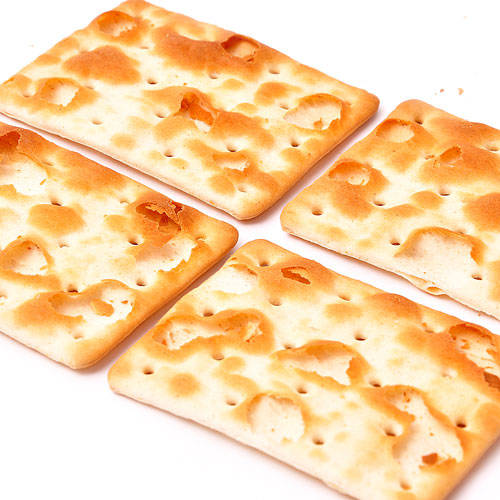
\includegraphics[width=1\linewidth]{traviatas}
        \caption[Traviatas]{Ejemplo 1.}
        \label{fig:traviatas_ej1}    
    \end{subfigure}
    %
    \hfill % llena el espacio entre figuras, para ocupar todo el ancho
    %
    \begin{subfigure}[b]{0.4\linewidth}
        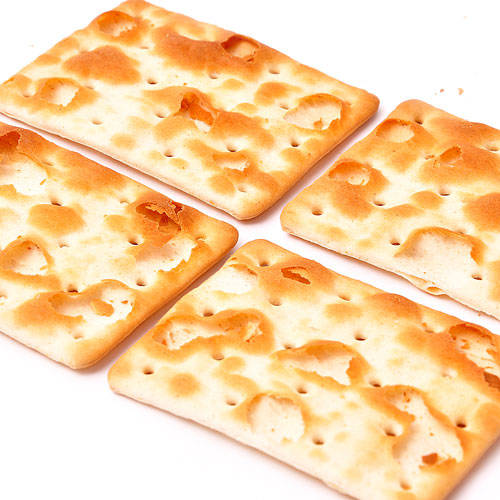
\includegraphics[width=1\linewidth]{traviatas}
        \caption[Traviatas]{Ejemplo 2.}
        \label{fig:traviatas_ej2}    
    \end{subfigure}
    %
    \caption[Traviatas]{Estas son galletas \nombre{Traviata} con burbujas quemadas.}
    \label{fig:traviatas}    
\end{figure}




% Ejemplo de 3 imágenes en línea
\begin{figure}
    \centering
    %
    \begin{subfigure}[b]{0.3\linewidth}
        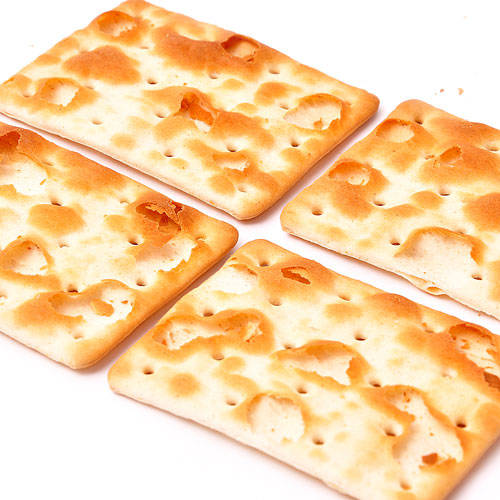
\includegraphics[width=1\linewidth]{traviatas}
        \caption[Traviatas]{Ejemplo 1.}  
    \end{subfigure}
    %
    \hfill % llena el espacio entre figuras, para ocupar todo el ancho
    %
    \begin{subfigure}[b]{0.3\linewidth}
        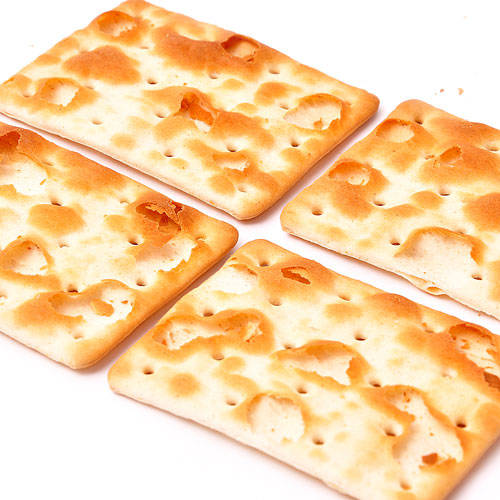
\includegraphics[width=1\linewidth]{traviatas}
        \caption[Traviatas]{Ejemplo 2.} 
    \end{subfigure}
    %
    \hfill % llena el espacio entre figuras, para ocupar todo el ancho
    %
    \begin{subfigure}[b]{0.3\linewidth}
        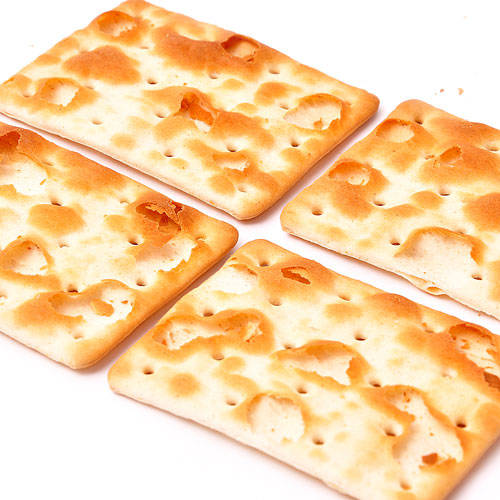
\includegraphics[width=1\linewidth]{traviatas}
        \caption[Traviatas]{Ejemplo 3.} 
    \end{subfigure}
    %
    \caption[Traviatas]{Estas son galletas \nombre{Traviata} con burbujas quemadas.}
    \label{fig:3traviatas}    
\end{figure}




% Ejemplo de cuatro subimágenes en dos filas
\begin{figure}
    \centering
    %
    \begin{subfigure}[b]{0.2\linewidth}
        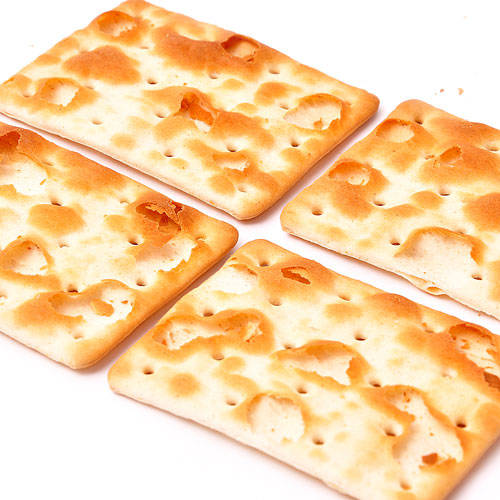
\includegraphics[width=1\linewidth]{traviatas}
        \caption[Traviatas]{Ejemplo 1.}  
    \end{subfigure}
    %
%    \hfill % llena el espacio entre figuras, para ocupar todo el ancho
    %
    \begin{subfigure}[b]{0.2\linewidth}
        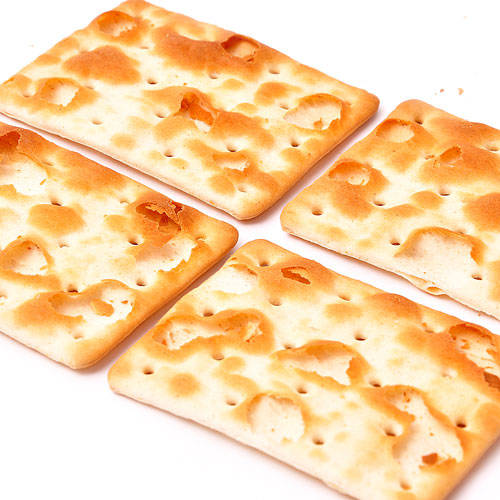
\includegraphics[width=1\linewidth]{traviatas}
        \caption[Traviatas]{Ejemplo 2.} 
    \end{subfigure}
    %
    \\ % salto de línea
    %
    \begin{subfigure}[b]{0.2\linewidth}
        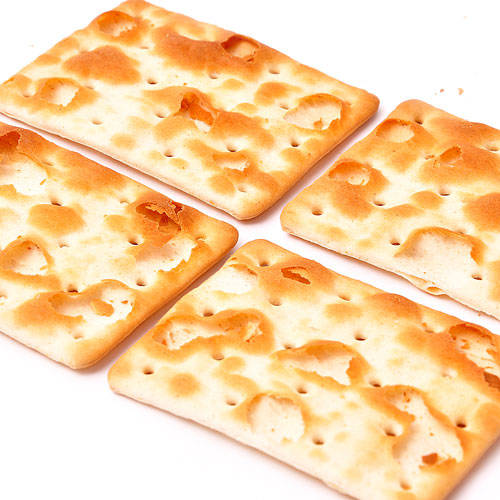
\includegraphics[width=1\linewidth]{traviatas}
        \caption[Traviatas]{Ejemplo 3.}  
    \end{subfigure}
    %
%    \hfill % llena el espacio entre figuras, para ocupar todo el ancho
    %
    \begin{subfigure}[b]{0.2\linewidth}
        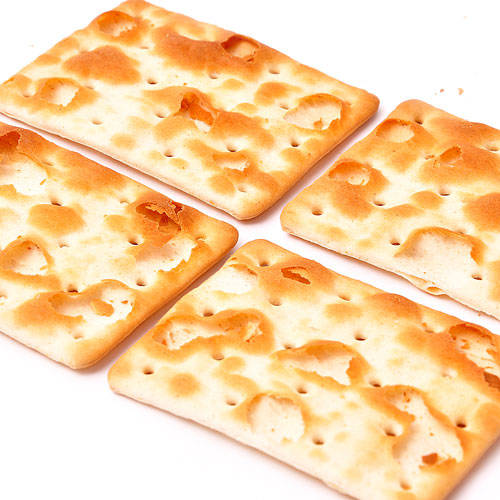
\includegraphics[width=1\linewidth]{traviatas}
        \caption[Traviatas]{Ejemplo 4.} 
    \end{subfigure}
    %
    \caption[Traviatas]{Estas son galletas \nombre{Traviata} con burbujas quemadas.}
    \label{fig:4traviatas}    
\end{figure}



% Ejemplo de cuatro subimágenes en dos filas, pero con más espacio horizontal y vertical
\begin{figure}
    \centering
    %
    \begin{subfigure}[b]{0.2\linewidth}
        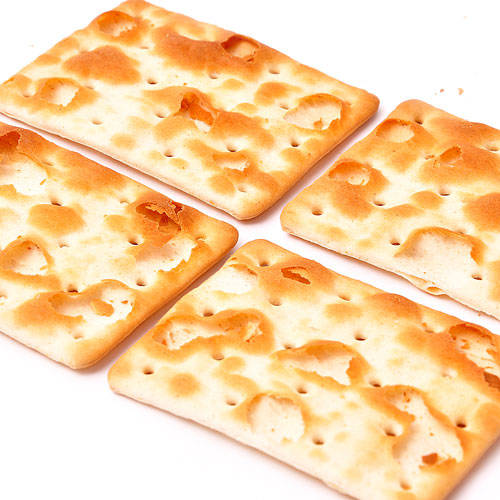
\includegraphics[width=1\linewidth]{traviatas}
        \caption[Traviatas]{Ejemplo 1.}  
    \end{subfigure}
    %
    \hspace{0.1\linewidth} % espacio horizontal
    %
    \begin{subfigure}[b]{0.2\linewidth}
        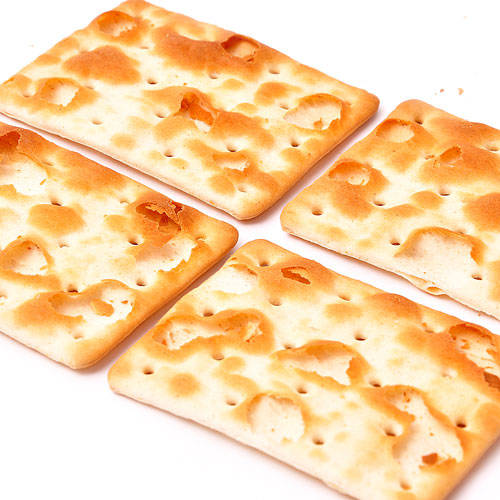
\includegraphics[width=1\linewidth]{traviatas}
        \caption[Traviatas]{Ejemplo 2.} 
    \end{subfigure}
    %
    \\ % salto de línea
    \vspace{0.1\linewidth} % espacio vertical
    %
    \begin{subfigure}[b]{0.2\linewidth}
        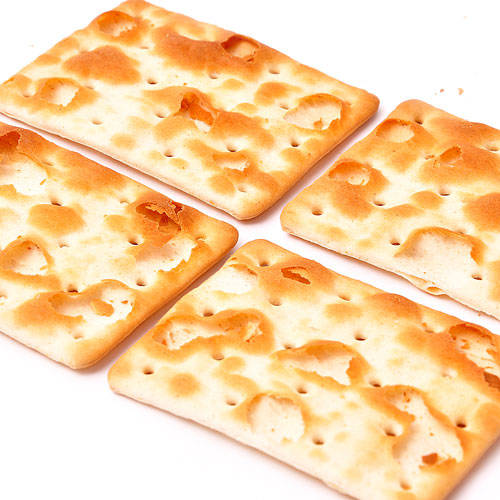
\includegraphics[width=1\linewidth]{traviatas}
        \caption[Traviatas]{Ejemplo 3.}  
    \end{subfigure}
    %
    \hspace{1em} % espacio horizontal
    %
    \begin{subfigure}[b]{0.2\linewidth}
        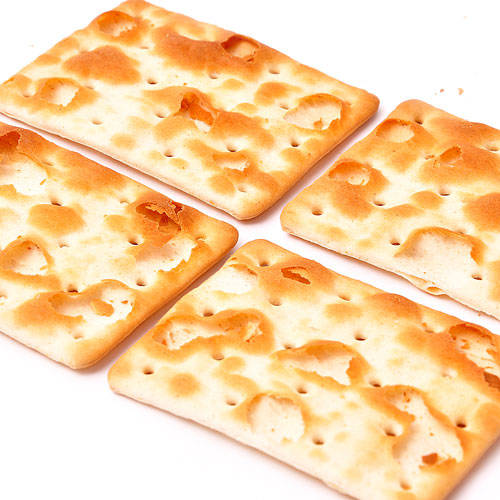
\includegraphics[width=1\linewidth]{traviatas}
        \caption[Traviatas]{Ejemplo 4.} 
    \end{subfigure}
    %
    \caption[Traviatas]{Estas son galletas \nombre{Traviata} con burbujas quemadas.}
    \label{fig:4traviatas_otras}    
\end{figure}




\minisec{Criollitas}

Este es un párrafo de las \nombre{Criollitas}.


\minisec{Mediatarde}

Este es un párrafo de las \nombre{Mediatarde}.


\paragraph{Hogareñas} Este párrafo referido a las galletas \nombre{Hogareñas} está hecho con \texttt{\textbackslash paragraph\{\}} en lugar de \texttt{\textbackslash minisec\{\}}. Es otra opción de encabezado menor. Probablemente sea mejor que \texttt{minisec}, para mantener uniformidad.

Y la \cref{tabla:tabladeejemplo} es una tabla de ejemplo.

\begin{table}[hbt]
    \centering
    \caption[Cultivos de almendra en Argentina en 2015]{cultivos de almendra en Argentina en 2015.~\autocite{iannamico:cultivo}}
    \label{tabla:tabladeejemplo}
    \begin{tabular}{@{}lr@{}}
        \toprule
        Provincia           & Superficie cultivada {[}Ha{]} \\ \cmidrule{1-2} % o \midrule
        Mendoza             & 2580                          \\
        San Juan            & 572                           \\
        La Rioja            & 498                           \\
        Salta               & 189                           \\
        Río Negro y Neuquén & 170                           \\
        Otras               & 200                           \\
        Total               & 4209                          \\ \bottomrule
    \end{tabular}
\end{table}


Acá un poco del uso de \nombre{SIUnitx} para el formato de números y unidades. \SI{30}{\kg},  \SI{80}{\percent}, \num{2015}, \num{40000}, \SI{800x600}{\pixel}, \num{640x480}, \ang{45}, \SIrange{10}{20}{\kilogram}, \SIlist{1;2;3}{\metre} , \SIrange{1}{10}{\degreeCelsius}, \SI{12.3(2)}{\kilogram}. También funciona en modo matemático:
$ \SI{15000}{\micro\gram} $




\pagebreak

Agrego por último unas ecuaciones de ejemplo. Se determinan a continuación la media circular y la desviación estándar circular, que se usaron como descriptores de color.~\autocite{estcirc}

% PREGUNTAR SI ECUACIÓN CON NÚMEROS. IMPLICARÍA QUE LAS DE LOS CLASIFICADORES TAMBIÉN TENGAN...
Sea un conjunto de $ n $ ángulos $ a_1, a_2, \dots, a_n $. Estos pueden interpretarse como $ n $ vectores $ \bm{v} $ de magnitud $ 1 $ y ángulos $ a_1, a_2, \dots, a_n $ respectivamente:
%
\begin{equation} \bm{v_n} = 1 e^{j a_n} \end{equation}
%
Si se convierten a coordenadas cartesianas, se tiene:
%
\begin{equation} \bm{v_n} = \cos(a_n) + j \sin(a_n) \end{equation}
%
Sumando los $ n $ vectores obtenemos el vector resultante $ \bm{a} $:
%
\begin{equation} \bm{a} = \sum_{1}^{n} \bm{v_n} = R e^{j \rho} \end{equation}
%
La \textbf{media circular} (o \textbf{ángulo medio} en este caso) es el ángulo $ \rho $ descripto por este vector resultante $ \bm{a} $.
%
La longitud media de los vectores $ \bm{v_n} $ se define como:
%
\begin{equation} \bar{R} = \frac{R}{n} \end{equation}
%
Y la \textbf{desviación estándar circular} como:
%
\begin{equation} S = \sqrt{\ln\left(\frac{1}{\bar{R}^2}\right)} = \sqrt{-2 \ln \left( \bar{R}^2 \right) } \end{equation}
\chapter{Introducción}



\section{Problemática y motivación}

La almendra es la fruta seca de mayor producción y consumo en el mundo.~\autocite{iannamico:frutossecos} Se comercializa con diversos grados de industrialización: con cáscara; pelada; blanqueada; en trozos; como harina; como aceite y como pasta, entre otros. El mercado mundial de las almendras está dominado en un \SI{80}{\percent} por dos principales productores: Estados Unidos y España. En \num{2015}, nuestro país tenía más de \num{4000} hectáreas cultivadas (ver tabla \ref{tabla:supcultivada}), siendo Mendoza la provincia de mayor superficie cultivada, seguida por San Juan y La Rioja. En \num{2013} se importaron más de \num{1800} toneladas de almendras para el consumo local —desde Chile y Estados Unidos—, mientras que se exportaron \num{33} toneladas a España, Paraguay y Uruguay.~\autocite{faostat}


\begin{table}[hbt]
\centering
\caption[Cultivos de almendra en Argentina en 2015]{cultivos de almendra en Argentina en 2015.~\autocite{iannamico:cultivo}}
\label{tabla:supcultivada}
\begin{tabular}{@{}lr@{}}
\toprule
Provincia           & Superficie cultivada {[}Ha{]} \\ \cmidrule{1-2} % o \midrule
Mendoza             & 2580                          \\
San Juan            & 572                           \\
La Rioja            & 498                           \\
Salta               & 189                           \\
Río Negro y Neuquén & 170                           \\
Otras               & 200                           \\
Total               & 4209                          \\ \bottomrule
\end{tabular}
\end{table}


El procesamiento mínimo para comercializar las almendras implica el descapotado y el pelado. El descapotado consiste en eliminar la cáscara externa o \enquote{capote} (exocarpio y mesocarpio del fruto); en el pelado se rompe la cáscara interna (endocarpio del fruto) para finalmente extraer la semilla. Este procesamiento es realizado mecánicamente por máquinas especializadas, pero puede provocar ligeros daños en algunos frutos. Posteriormente se realiza un proceso de clasificación o filtrado en el cual se eliminan restos de cáscaras, almendras dañadas y cualquier objeto extraño. Esta clasificación es habitualmente realizada mediante clasificadores ópticos, máquinas de alta tecnología y costo que mediante iluminadores, cámaras y eyectores de aire, separan los productos buenos de los malos y la basura.

En la región, y particularmente en la provincia de San Juan, la producción está centrada en pequeñas y medianas empresas agroindustriales. Hoy en día algunos productores optan por vender las almendras con cáscara; serán otros quienes les den, al pelarlas, mayor valor agregado. Otros productores sí realizan esa etapa de procesado, separando las almendras buenas de forma manual, lo cual requiere mano de obra especializada y muchas horas de trabajo; el promedio por operario es de entre \num{15} y \SI{30}{\kg} por jornada. La escasez de mano de obra especializada (debido a lo rutinario de la tarea) impacta en los costos de producción, pero estos productores no pueden afrontar los costos de adquirir una máquina clasificadora óptica.

El \nombre{Proyecto de Desarrollo Tecnológico y Social} (\nombre{PDTS}) \enquote{Diseño e implementación de una estrategia de clasificación óptica de almendras para pequeños productores} es una iniciativa impulsada por la \nombre{Universidad Nacional de San Juan} (\nombre{UNSJ}) y la \nombre{Secretaría de Ciencia, Tecnología e Innovación} del \nombre{Gobierno de San Juan} (\nombre{SECITI}) que pretende, a largo plazo, desarrollar una clasificadora óptica de almendras destinada al sector \nombre{MiPyME} agroindustrial de la región del Nuevo Cuyo.~\autocite{pdts} Para ello hay que diseñar, construir y probar todas las partes mecánicas, electrónicas y de software de la máquina, como así también los procesos que en ella se realizan y cómo se integran a los procesos existentes. Debe ser de bajo costo y ser al menos tan eficiente como un operario humano que clasifica manualmente.

Este trabajo es un pequeño aporte inicial a ese \nombre{PDTS}, y aborda el diseño e implementación de un sistema de visión artificial para la clasificación de almendras




\section{La almendra}
La almendra es el fruto (tipo drupa) del árbol llamado almendro (\textit{Prunus dulcis [Mill.] D.A.Webb}). Una drupa es un fruto monospermo de mesocarpio carnoso, coriáceo o fibroso, que rodea a un endocarpio leñoso (carozo o hueso) con una sola semilla en su interior. Otras drupas son el durazno, la cereza, la aceituna y el café.

En la almendra el mesocarpio y el exocarpio forman la parte más blanda, correosa, del fruto; se conoce como cáscara o capote (en inglés: \ingles{hull}). El endocarpio (ver figura \ref{fig:partesalmendra}) es la cáscara dura, carozo o hueso (en inglés: \ingles{shell}). En la parte interna del carozo está la semilla (\ingles{kernel}) dicotiledónea, que es lo que vulgarmente se conoce como almendra. Esta se puede dividir longitudinalmente en dos mitades llamadas cotiledones. La semilla tiene una piel marrón que la rodea: el tegumento. Para diferenciar las partes de la semilla, llamaremos \enquote{carne} a la parte blanca que está dentro del tegumento.


\begin{figure}[hbtp]
\centering
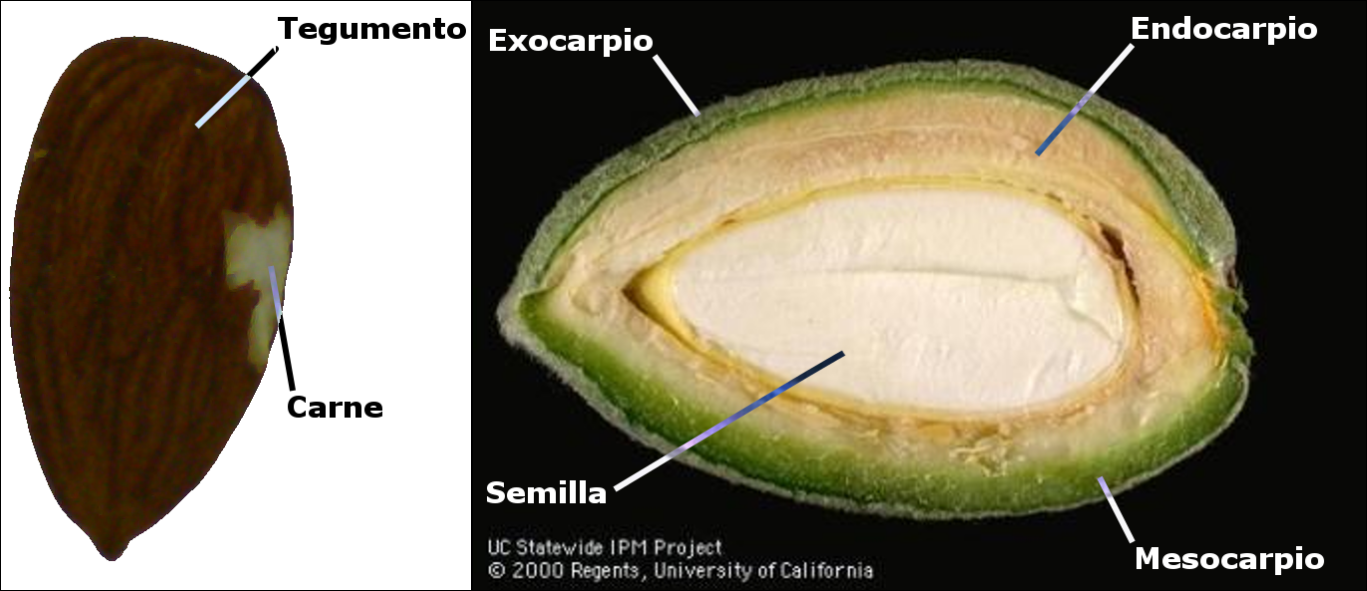
\includegraphics[width=\imagengrande]{almendra_partes_1_2}
\caption[Partes de una almendra]{partes de una almendra. Izquierda: semilla; derecha: corte de un fruto completo.~\autocite[][]{imagenes:interioralmendra}}
\label{fig:partesalmendra}
\end{figure}




\section{Normas}
Existen normas que regulan el comercio de almendras peladas (sin cáscara). Hay tres normas que fueron útiles para definir los defectos a encontrar: 
\begin{enumerate}
\item la Resolución \num{1352/1967} (capítulos XV y XIX) de la antigua \nombre{Secretaría de Agricultura y Ganadería de la República Argentina}, hoy bajo la órbita del \nombre{Servicio Nacional de Sanidad y Calidad Agroalimentaria} (\nombre{SENASA});~\autocite{standards:res1352}

\item el \enquote{Estándar estadounidense para la calidad de almendras peladas}, elaborado por el \nombre{Departamento de Agricultura} de ese país (\nombre{USDA});~\autocite{standards:usda}

\item el \enquote{Estándar DDP-06 acerca de la comercialización y control de calidad comercial de semillas de almendra}, elaborado por la \nombre{Comisión Económica de las Naciones Unidas para Europa} (\nombre{UNECE}).~\autocite{standards:unece}

\end{enumerate}

Los tres documentos definen rasgos generales sobre los bienes a comercializar, y caracterizan defectos a encontrar, como \enquote{almendras partidas}, \enquote{almendras dobles}, \enquote{moho}, \enquote{fragmento} y otros. Por último, establecen clases de calidad, cada una con distinta tolerancia a defectos o variaciones.

Las normas de \nombre{UNECE} y \nombre{USDA} son más explícitas a la hora de definir los defectos que la norma de \nombre{SENASA}. El \nombre{Código Alimentario Argentino} replica en su capítulo XI una versión abreviada de la Resolución \num{1352/1967}.~\autocite{codigoalimentario}



\section{Soluciones existentes}
Existen en el mercado máquinas capaces de resolver el problema con el mismo enfoque; se denominan máquinas de clasificación óptica o seleccionadoras ópticas (en inglés es común denominarlas como  \ingles{optical sorting machines}, y no \ingles{optical classification machines}). Se utilizan, en general, luego de etapas de filtrado mecánico. Estas máquinas pueden usarse para una gran cantidad de frutos; el fabricante ajusta sus parámetros y añade o quita componentes según el fruto a clasificar y el presupuesto del comprador. 

La estructura de la gran mayoría de ellas consiste de:

\begin{enumerate}
\item Una cinta transportadora o plataforma vibradora, que mueve los frutos.
\item Un tobogán o tubo que guía los frutos hacia un espacio de caída libre.
\item Una o más cámaras que capturan imágenes desde uno o ambos lados del objeto.
\item Eyectores que soplan los objetos malos.
\item Salidas de objetos malos y objetos buenos.
\end{enumerate}
A modo de ejemplo, la figura \ref{fig:diagramamaquina} muestra un esquema de funcionamiento de una clasificadora \nombre{Tomra Nimbus}.



\begin{figure}[hbtp]
\centering
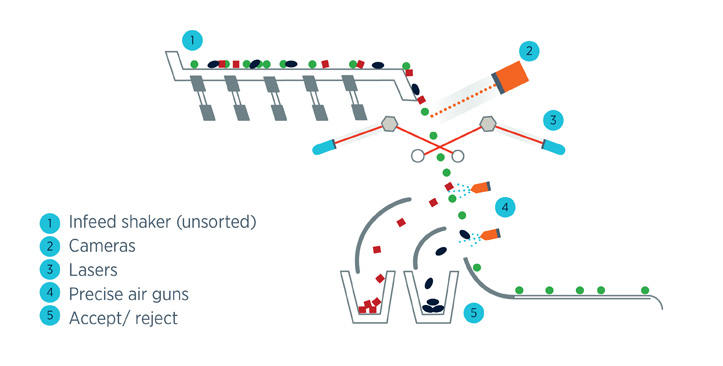
\includegraphics[width=\imagengrande]{tomra_nimbus_diagrama}
\caption[Diagrama de funcionamiento de una máquina comercial]{diagrama de funcionamiento de una máquina \nombre{Tomra Nimbus}.~\autocite{imagenes:nimbusdiagrama}}
\label{fig:diagramamaquina}
\end{figure}
%TODO: Vectorizar.


La figura \ref{fig:salidamaquina} muestra la salida típica de una máquina clasificadora. Los defectos que pueden detectarse están determinados por el software de las máquinas y por el sistema de visión que tienen. Respecto a esto último, pueden tener cámaras e iluminadores en el espectro visible, en ultravioleta y en infrarrojo, que permiten detectar:
\begin{itemize}
\item Problemas de forma;
\item Problemas de color;
\item Hongos y toxinas superficiales;
\item Objetos extraños.
\end{itemize}



\begin{figure}[hbtp]
\centering
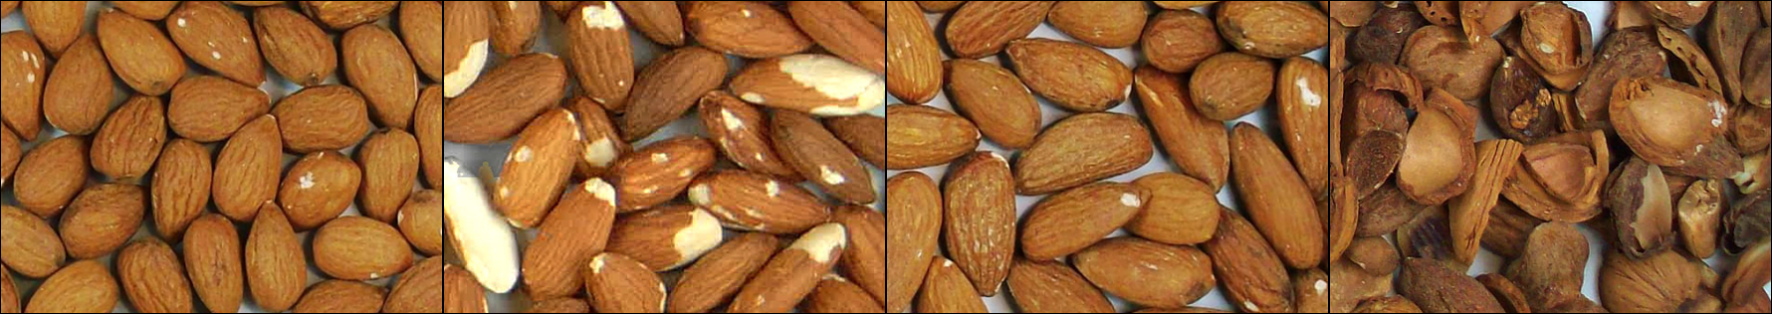
\includegraphics[width=\imagengrande]{almendras_clasificadora_a}
\caption[Salida de una máquina clasificadora comercial]{salida de una máquina clasificadora comercial. De izquierda a derecha: almendras aceptadas; rechazadas por astilladas o raspadas; rechazadas por tamaño; rechazadas por ser cáscaras, almendras manchadas o podridas.~\autocite{imagenes:almendrasclasificadas}}
\label{fig:salidamaquina}
\end{figure}


La mayoría usa sensores CCD e iluminadores led, pero algunas incorporan luz láser y los sensores correspondientes, para analizar ciertos defectos. 

Algunas empresas que fabrican estas máquinas son \nombre{Tomra}, \nombre{Bühler}, \nombre{Cimbria} y \nombre{Key Technology}; algunas de sus máquinas se muestran en la figura \ref{fig:maquinas}. Hay muchas más que fabrican máquinas simples que solo analizan el color. No se encontró información respecto a la precisión de las máquinas. Su capacidad depende del producto a analizar y los defectos a encontrar, pero es mayor a \SI{0,5}{toneladas/hora}, pudiendo alcanzar \SI{15}{toneladas/hora}.

En nuestro país, las máquinas de la familia \nombre{Sortex} de \nombre{Bühler} tienen un costo que oscila entre los \SI{100000}{USD} y los \SI{300000}{USD} ---alrededor de \SI{1780000}{ARS} y \SI{5340000}{ARS} respectivamente, en agosto de 2017---, dependiendo de los defectos a remover y la capacidad de producción (entre \num{2} y \SI{15}{toneladas/hora}). En función de esto varían el tipo y cantidad de cámaras (entre dos y veinte).\footnote{Según comunicación por correo electrónico con \nombre{Walter Tosco} de \nombre{Bühler Sortex Argentina} (\url{http://sortex.com.ar}).}



\begin{figure}[hbtp]
\centering
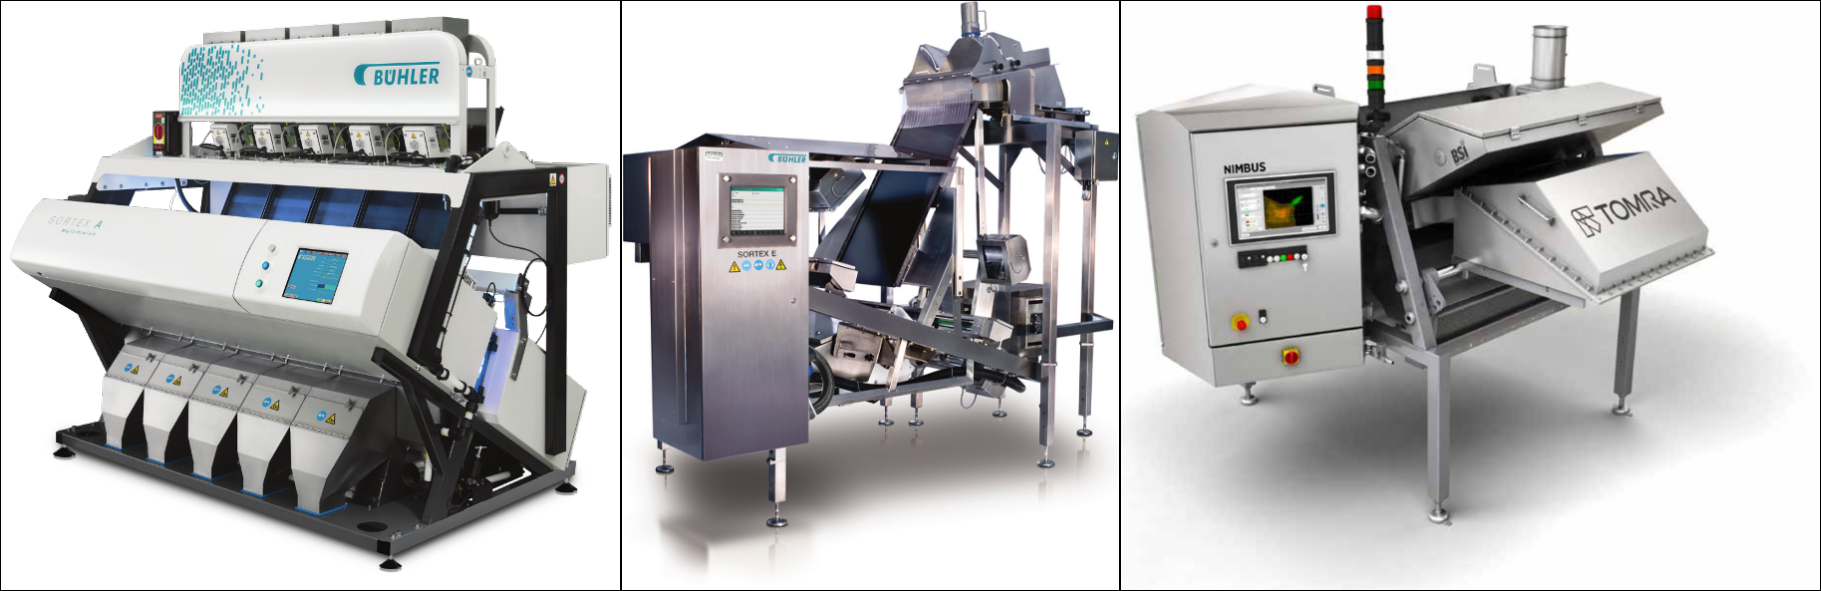
\includegraphics[width=\imagengrande]{maquinas}
\caption[Máquinas clasificadoras]{máquinas clasificadoras ópticas. De izquierda a derecha: \nombre{Bühler Sortex A}, \nombre{Bühler Sortex E}, \nombre{Tomra Nimbus}.~\autocite{imagenes:maquinasbuhler,imagenes:maquinastomra}}
\label{fig:maquinas}
\end{figure}



\section{Propuesta}
En este trabajo se quisieron abordar tres áreas específicas de la máquina: el software de clasificación, el proceso de captura y el sistema de desplazamiento de las almendras. Una vez comenzado el trabajo se hizo evidente que el sistema de visión artificial necesario no es independiente de los mecanismos de traslación y eyección de objetos. Dado que estos últimos no están definidos todavía (y dependen de otras partes del proceso), adoptar un subsistema de visión único, sin considerar posibles limitaciones a las otras partes del sistema clasificador, es una decisión que probablemente implicaría problemas en futuras etapas. Es por esto que se decidió:

\begin{enumerate}
\item Hacer pruebas cortas de posibles sistemas de visión, lo más genéricos posibles.
\item Tomar el que mejor funcione (según algún criterio) y utilizarlo para generar un gran conjunto de imágenes.
\end{enumerate}

Este conjunto de imágenes se usa para evaluar la efectividad que tienen diversos descriptores o predictores para clasificar los objetos que ingresen al sistema. Algunos de los descriptores usados son propuestos en la literatura revisada, mientras que otros surgen de nuestro análisis del problema de clasificación. Análogamente, se prueban diversas formas de identificar de forma unívoca las posiciones y límites de los objetos en las imágenes —tarea conocida como segmentación—.

El conjunto de imágenes fue generado a partir de almendras y otros objetos provistos por un productor local. Se utilizaron (parcialmente) las normas de \nombre{UNECE} como verdad o patrón de referencia, para definir los defectos a buscar en las almendras y para comparar los resultados obtenidos. Algunos valores de referencia, como el color y el tamaño, se determinan a partir de la muestra ya que son características que varían naturalmente entre especies y cosechas.



\section{Herramientas y materiales}\label{intro:herramientasymateriales}
Se resumen a continuación algunas de las herramientas y materiales que se utilizaron en este trabajo. Se extenderá su descripción y forma de uso en secciones posteriores.

\begin{enumerate}
\item Cámara web \nombre{Genius eFace 2050AF}.
\item Muestras  de almendras y otros objetos, provistos por el productor.
\item \nombre{Matlab R2015b}~\autocite{soft:matlab}. Se decidió hacer el desarrollo de los algoritmos en \nombre{Matlab}, ya que es una herramienta versátil; buena para la experimentación y el análisis; y de amplio uso en el \nombre{Instituto de Automática} (\nombre{INAUT}), donde probablemente se continúe el desarrollo del sistema.

Cajas de herramientas usadas:
	\begin{enumerate}
	\item {\nombre{Image Processing Toolbox}}
	\item {\nombre{Computer Vision System Toolbox}}
	\item {\nombre{Image Acquisition Toolbox}}
	\item {\nombre{Statistics and Machine Learning Toolbox}}
	\end{enumerate}
Otros:
	\begin{enumerate}
	\item {\nombre{Matlab Support Package for USB Webcams}}
	\item \nombre{YAMLMatlab}, para trabajar con archivos YAML de configuración de parámetros~\autocite{soft:yamlmatlab}
	\item \nombre{MBeautifier}, para uniformar el formato del código~\autocite{soft:mbeautifier}
	\item \nombre{multic} ({\nombre{Confusion Matrix and its Derivations}})~\autocite{soft:multic}
	\item {\nombre{Balu Toolbox for Matlab}}~\autocite{soft:balu}
	\end{enumerate}
\item \nombre{GIMP 2.8.18}:  Programa de edición de imágenes utilizado como complemento a \nombre{Matlab} para el diseño de algoritmos y análisis de las imágenes disponibles. Se usó también el complemento \nombre{G’MIC 1.79} para el procesamiento.~\autocite{soft:gimp,soft:gmic}
\item \nombre{KNIME 3.3.2}: Programa de minería de datos usado para comparar resultados.~\autocite{soft:knime}
\item Perfiles metálicos y accesorios; poliestireno de alto impacto; madera MDF; vidrios y espejos, para la construcción de un prototipo de estructura.
\item Tiras de leds, una fuente conmutada y materiales eléctricos, para la construcción de luminarias.
\end{enumerate}

\chapter{Resultados}

En base al desempeño observado durante el desarrollo y prueba de cada una de las etapas de preprocesamiento, segmentación y clasificación, elegimos algunas de ellas para formar parte del algoritmo a evaluar. El algoritmo es (ver figura \ref{fig:esquemaalgoritmofinal}): 
%
\begin{enumerate}
\item Preprocesador: suavizado gaussiano
\item Segmentador: basado en imagen retroiluminada
\item Clasificador: según altura
\item Clasificador: según extensión de la caja envolvente
\item Clasificador: según relación de aspecto de los ejes de una elipse ajustada
\item Clasificador: según área sin tegumento (raspaduras) a partir de canales H, S y V
\item Clasificador: según media de color (canal H)
\item Clasificador: según desviación de color (canal H)
\item Clasificador: según media de color (canal a*)
\item Clasificador: según media de color (canal b*)
\item Clasificador: según solidez
\end{enumerate}

\begin{figure}[hbtp]
\centering
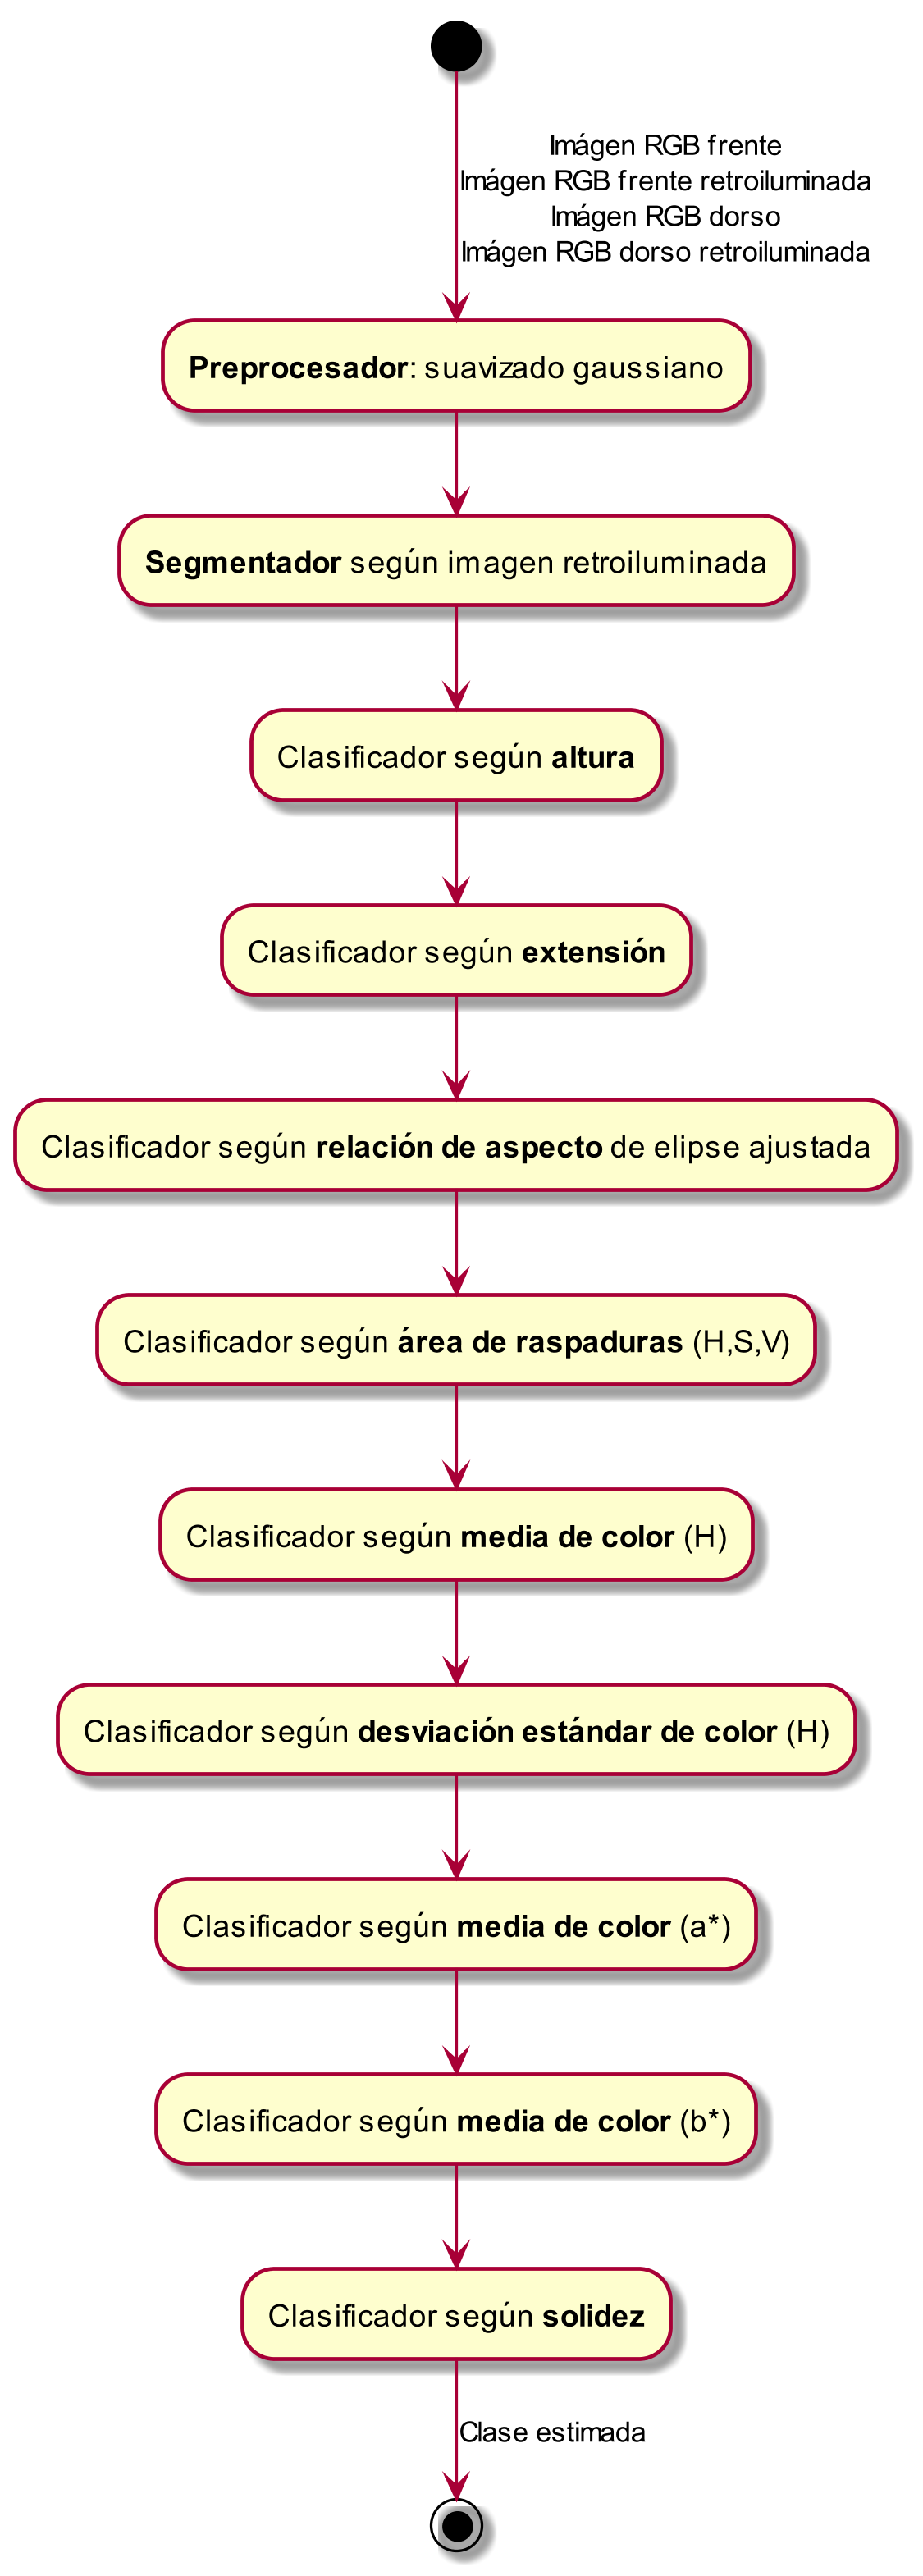
\includegraphics[width=\textwidth,height=0.9\textheight,keepaspectratio]{clasificadorfinal}
%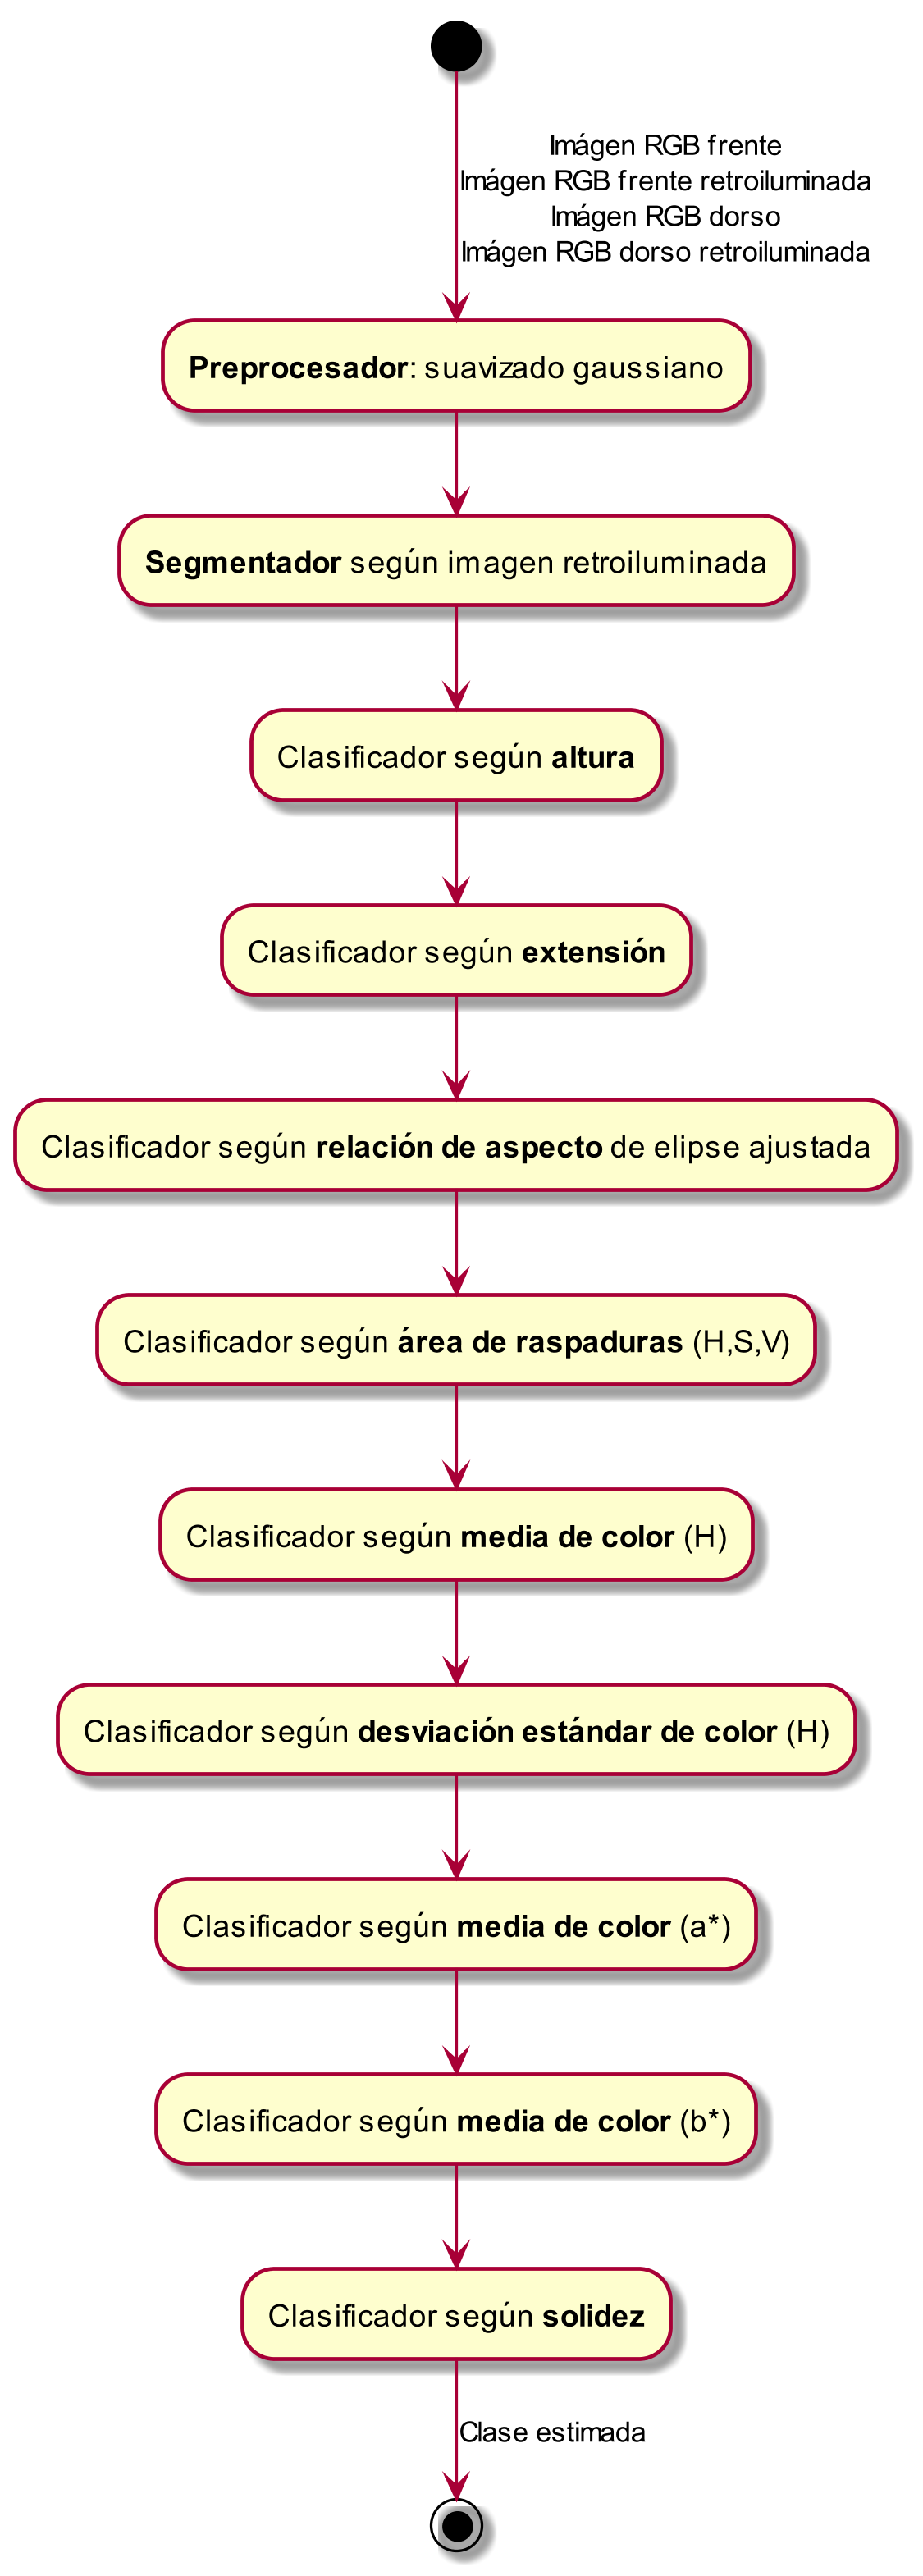
\includegraphics[scale=\escaladiagramas]{clasificadorfinal}
\caption[Etapas del algoritmo final]{etapas del algoritmo final.}
\label{fig:esquemaalgoritmofinal}
\end{figure}


Quedó fuera el clasificador según la relación de aspecto de la caja envolvente, porque es muy similar al de la relación de aspecto de la elipse ajustada. No se usó el clasificador según el área de arrugas por su mal desempeño general. El clasificador según área de raspaduras a partir de los canales H, S y V es mejor que el que solo usa S.

Es importante notar que los clasificadores según características de color (etapas \numlist{7;8;9;10}) realizan sus medidas a partir de los datos que están en las zonas con tegumento\footnote{También se pueden usar con la máscara del objeto completo.}; esta está determinada por la máscara creada por el clasificador según raspaduras y por tanto las medidas solo serán correctas en el caso de almendras y objetos de colores similares a los de las almendras.

Los parámetros de funcionamiento de cada clasificador fueron ajustados heurísticamente durante su desarrollo\footnote{Los valores se pueden ver en los archivos de clase correspondientes o en cualquier archivo \texttt{parametros\_efectivos*.yml} en las carpetas de experimentos.}, analizando su desempeño general o específico para el defecto que buscaban encontrar. Los parámetros que determinan los límites de clasificación se ajustarán según diferentes estrategias, como se menciona más adelante.





\section{Metodología de ajuste y evaluación}




\subsection{Evaluación}
La evaluación se hará sobre el conjunto \nombre{set3}, para dos casos de trabajo distintos:
\begin{enumerate}
\item Contemplando las tres clases del conjunto: Primera, Mala y No Almendra.
\item Simplificando a solo dos clases: Buena (clase Primera) y Mala (clase Mala y clase No Almendra). Esto se justifica porque no encontramos criterios confiables para separar las clases Mala y No Almendra.
\end{enumerate}

La evaluación se hará sobre el conjunto de evaluación —un \SI{20}{\percent} del total—, mientras que el ajuste de los parámetros de clasificación de cada etapa se hará según los valores de los descriptores sobre el conjunto de entrenamiento —el restante \SI{80}{\percent}—. Ver \ref{captura:particionypreprocesado}.

Los resultados de nuestro clasificador serán contrastados contra los obtenidos por algoritmos de aprendizaje automático en \nombre{KNIME} y \nombre{Matlab Classification Learner} (ver \ref{intro:herramientasymateriales}) a partir de los mismos descriptores. De la herramienta de \nombre{Matlab} se usarán algunas de las configuraciones por defecto disponibles en la galería de clasificadores (usando validación cruzada con las mismas proporciones ---\SI{80}{\percent} de entrenamiento y \SI{20}{\percent} de validación--- que usamos para dividir el conjunto \nombre{set3}):
%
\begin{itemize}
\item Un árbol de decisiones simple, con menos de cuatro particiones (\ingles{splits})
\item Un árbol de decisiones de tamaño medio, con menos de veinte particiones (\ingles{splits})
\item Una máquina de vector soporte o máquina de soporte vectorial (SVM) lineal
\item Una SVM de núcleo cuadrático
\item Una SVM de núcleo cúbico
\item Un claificador de k vecinos cercanos (\ingles{k-nearest neighbours}, KNN), con un vecino
\item Un clasificador KNN con diez vecinos
\item \ingles{Boosted Trees}: un arreglo de clasificadores (árboles de decisión) optimizados con el algoritmo \nombre{Adaboost}.
\end{itemize}

En \nombre{KNIME} dividimos el conjunto \nombre{set3} en dos subconjuntos (\SI{80}{\percent} de entrenamiento y \SI{20}{\percent} de validación) y probamos dos clasificadores, con las opciones por defecto:
%
\begin{itemize}
\item Un árbol de decisión con menos de diez particiones
\item Un clasificador KNN con tres vecinos
\end{itemize}




\subsection{Métrica}
La métrica de evaluación de cada algoritmo será la exactitud global (\ingles{overall accuracy}) del sistema:
%
\begin{equation} \text{Exactitud global} = \frac{\text{elementos clasificados correctamente}}{\text{total de elementos}} \end{equation}

Esta se puede usar tanto para el caso de clasificación multiclase (Primera, Mala y No Almendra) como para la simplificación binaria (Buena y Mala).

Para este último caso, las proporciones de Buena y Mala son muy similares y por tanto no existe error de (alta) exactitud causado por clases desproporcionadas. Dado esto, un clasificador binario aleatorio tendrá una exactitud igual a la proporción inicial de las clases, cercana al \SI{50}{\percent}; por tanto \SI{50}{\percent} es la base de referencia para la clasificación binaria.




\subsection{Ajuste}
Los parámetros de clasificación (máximos y mínimos tolerados) de cada etapa clasificadora fueron ajustados siguiendo distintas estrategias, en base a los valores de los descriptores calculados para las almendras clasificadas como de Primera clase dentro del conjunto de entrenamiento (ver tabla \ref{tabla:valoresdescriptores}).

Las estrategias son:

\begin{description}
\item [Máximos y mínimos (Maxmin)] Los máximos y mínimos de tolerancia para cada clasificador son los máximos y mínimos medidos en las almendras de Primera clase del conjunto de entrenamiento.
\item [90\,\%] Se supone que cada descriptor sigue una distribución normal, con media $ \mu $ y desviación estándar $ \sigma $; la muestra es el conjunto almendras de Primera clase dentro del conjunto de entrenamiento. Se ajustan los máximos a $ \mu + 1,64 \sigma $ y los mínimos a $ \mu - 1,64\sigma $, lo cual abarca el \SI{90}{\percent} de los datos en una distribución normal.
\item [95\,\%] Análoga a la estrategia anterior, pero con un rango $ \left[ \mu - 2\sigma, \mu + 2\sigma \right] $, que abarca al \SI{95}{\percent} de los datos en una distribución normal.
\item [99\,\%] Análoga a las anteriores, pero con un rango $ \left[ \mu - 2,6\sigma, \mu + 2,6\sigma \right] $, que abarca al \SI{99}{\percent} de los datos en una distribución normal.
\item [Heurística 1 (H1)] Todos los límites igual a los de \textbf{\nombre{95\,\%}}, menos la tolerancia del área máxima de raspaduras; esta es la que determina la norma de \nombre{UNECE}: el área de un círculo de \SI{3}{\mm} de diámetro (aproximadamente \SI{7}{\mm\squared}).
\item [Heurística 2 (H2)] Análoga a \textbf{\nombre{Heurística 1}} pero usando los límites de \textbf{\nombre{99\,\%}}.
\end{description}

%\afterpage{%
%    \clearpage% Flush earlier floats (otherwise order might not be correct)
%    \thispagestyle{empty}% empty page style (?)
%    \begin{landscape}% Landscape page
%\begin{table}[htb]
%%\tymin=2cm
%\tiny
%\centering
%\caption{Características de los valores de los descriptores para las almendras de clase Buena (Primera) del conjunto de entrenamiento.}
%\label{tabla:valoresdescriptores}
%\begin{tabulary}{17cm}{lRRRRRRRRR}
%	\toprule
%	                      &                                                                                                                                                                   \multicolumn{9}{c}{\textbf{Descriptores}}                                                                                                                                                                    \\ \cmidrule{2-10}
%	\textbf{Medidas}      & \textbf{Altura [\si{\pixel}]} & \textbf{Extensión [\si{\pixel\squared}/\si{\pixel\squared}]} & \textbf{Relación de aspecto [\pixel/\pixel]} & \textbf{Área de raspaduras [\si{\mm\squared}]} & \textbf{Media de H [\si{\degree}]} & \textbf{Desviación estándar de H [\si{\degree}]} & \textbf{Media a*} & \textbf{Media b*} & \textbf{Solidez [\si{\pixel\squared}/\si{\pixel\squared}]} \\ \midrule
%	\textbf{máximo}          & 583,50                   & 0,774                                                              & 0,643                                    & 6,81                                                   & 34,48                       & 10,48                             & 17,48             & 30,72             & 0,9955                                                           \\
%	\textbf{mínimo}          & 428,50                   & 0,727                                                              & 0,444                                    & 0,00                                                   & 21,53                       & 3,52                              & 5,13              & 6,47              & 0,9837                                                           \\
%	                      &                          &                                                                    &                                          &                                                        &                             &                                   &                   &                   &  \\
%	$ \bm{\mu} $        & 510,14                   & 0,750                                                              & 0,553                                    & 0,46                                                   & 27,85                       & 4,94                              & 12,37             & 21,13             & 0,9931                                                           \\
%	$ \bm{\sigma} $   & 32,62                    & 0,011                                                              & 0,029                                    & 1,25                                                   & 2,29                        & 0,78                              & 1,78              & 5,00              & 0,0014                                                           \\
%	                      &                          &                                                                    &                                          &                                                        &                             &                                   &                   &                   &  \\
%	$ \bm{\mu+1,64\sigma} $ & 563,64                   & 0,767                                                              & 0,600                                    & 2,52                                                   & 31,60                       & 6,21                              & 15,30             & 29,33             & 0,9953                                                           \\
%	$ \bm{\mu-1,64\sigma} $ & 456,64                   & 0,732                                                              & 0,505                                    & -1,59                                                  & 24,10                       & 3,66                              & 9,45              & 12,94             & 0,9908                                                           \\
%	\textbf{}             &                          &                                                                    &                                          &                                                        &                             &                                   &                   &                   &  \\
%	$ \bm{\mu+2\sigma} $    & 575,38                   & 0,771                                                              & 0,610                                    & 2,97                                                   & 32,42                       & 6,49                              & 15,94             & 31,13             & 0,9958                                                           \\
%	$ \bm{\mu-2\sigma} $    & 444,90                   & 0,729                                                              & 0,495                                    & -2,04                                                  & 23,28                       & 3,38                              & 8,81              & 11,14             & 0,9903                                                           \\
%	\textbf{}             &                          &                                                                    &                                          &                                                        &                             &                                   &                   &                   &  \\
%	$ \bm{\mu+2,6\sigma} $  & 594,95                   & 0,777                                                              & 0,628                                    & 3,72                                                   & 33,79                       & 6,96                              & 17,01             & 34,13             & 0,9966                                                           \\
%	$ \bm{\mu-2,6\sigma} $  & 425,32                   & 0,722                                                              & 0,477                                    & -2,79                                                  & 21,91                       & 2,91                              & 7,74              & 8,14              & 0,9895                                                           \\ \bottomrule
%\end{tabulary}
%\end{table}
%    \end{landscape}
%    \clearpage% Flush page
%}





\begin{table}[htb]
%\tymin=2cm
%\scriptsize
\footnotesize
\centering
\caption[Características de los valores de los descriptores para las almendras de clase Buena (Primera) del conjunto de entrenamiento]{características de los valores de los descriptores para las almendras de clase Buena (Primera) del conjunto de entrenamiento.}
\label{tabla:valoresdescriptores}
\begin{tabulary}{0.97\textwidth}{lRRRRRRrrR}
	\toprule
	                      &                                                                                                                                                                   \multicolumn{9}{c}{\textbf{Descriptores}}                                                                                                                                                                    \\ \cmidrule{2-10}
	\textbf{Medidas}      & {\hbox{Altura} [\si{\pixel}]} & {\hbox{Extensión} [\si{\pixel\squared}/\si{\pixel\squared}]} & {Relación de aspecto [\pixel/\pixel]} & {Área de raspaduras [\si{\mm\squared}]} & {\hbox{Media} de H [\si{\degree}]} & {Desv. Est. de H [\si{\degree}]} & {\hbox{Media} a*} & {\hbox{Media} b*} & {\hbox{Solidez} [\si{\pixel\squared}/\si{\pixel\squared}]} \\ \midrule
	\textbf{máximo}          & 583,50                   & 0,774                                                              & 0,643                                    & 6,81                                                   & 34,48                       & 10,48                             & 17,48             & 30,72             & 0,9955                                                           \\
	\textbf{mínimo}          & 428,50                   & 0,727                                                              & 0,444                                    & 0,00                                                   & 21,53                       & 3,52                              & 5,13              & 6,47              & 0,9837                                                           \\
	                      &                          &                                                                    &                                          &                                                        &                             &                                   &                   &                   &  \\
	$ \bm{\mu} $        & 510,14                   & 0,750                                                              & 0,553                                    & 0,46                                                   & 27,85                       & 4,94                              & 12,37             & 21,13             & 0,9931                                                           \\
	$ \bm{\sigma} $   & 32,62                    & 0,011                                                              & 0,029                                    & 1,25                                                   & 2,29                        & 0,78                              & 1,78              & 5,00              & 0,0014                                                           \\
	                      &                          &                                                                    &                                          &                                                        &                             &                                   &                   &                   &  \\
	$ \bm{\mu+1,64\sigma} $ & 563,64                   & 0,767                                                              & 0,600                                    & 2,52                                                   & 31,60                       & 6,21                              & 15,30             & 29,33             & 0,9953                                                           \\
	$ \bm{\mu-1,64\sigma} $ & 456,64                   & 0,732                                                              & 0,505                                    & -1,59                                                  & 24,10                       & 3,66                              & 9,45              & 12,94             & 0,9908                                                           \\
	\textbf{}             &                          &                                                                    &                                          &                                                        &                             &                                   &                   &                   &  \\
	$ \bm{\mu+2\sigma} $    & 575,38                   & 0,771                                                              & 0,610                                    & 2,97                                                   & 32,42                       & 6,49                              & 15,94             & 31,13             & 0,9958                                                           \\
	$ \bm{\mu-2\sigma} $    & 444,90                   & 0,729                                                              & 0,495                                    & -2,04                                                  & 23,28                       & 3,38                              & 8,81              & 11,14             & 0,9903                                                           \\
	\textbf{}             &                          &                                                                    &                                          &                                                        &                             &                                   &                   &                   &  \\
	$ \bm{\mu+2,6\sigma} $  & 594,95                   & 0,777                                                              & 0,628                                    & 3,72                                                   & 33,79                       & 6,96                              & 17,01             & 34,13             & 0,9966                                                           \\
	$ \bm{\mu-2,6\sigma} $  & 425,32                   & 0,722                                                              & 0,477                                    & -2,79                                                  & 21,91                       & 2,91                              & 7,74              & 8,14              & 0,9895                                                           \\ \bottomrule
\end{tabulary}
\end{table}





%\begin{table}[htb]
%\centering
%\caption{Características de los valores de los descriptores para las almendras de clase Buena (Primera) del conjunto de entrenamiento.}
%\label{tabla:valoresdescriptores}
%\begin{tabular}{@{}llllllllll@{}}
%	\toprule
%	                      &                                                                                                                                                                   \multicolumn{9}{c}{\textbf{Descriptores}}                                                                                                                                                                    \\ 
%	\textbf{Medidas}      & \textbf{Altura [\si{\pixel}]} & \textbf{Extensión [\si{\pixel\squared}/\si{\pixel\squared}]} & \textbf{Relación de aspecto [\pixel/\pixel]} & \textbf{Área de raspaduras [\si{\mm\squared}]} & \textbf{Media de H [\si{\degree}]} & \textbf{Desviación estándar de H [\si{\degree}]} & \textbf{Media a*} & \textbf{Media b*} & \textbf{Solidez [\si{\pixel\squared}/\si{\pixel\squared}]} \\ \midrule
%	\textbf{máximo}          & 583,50                   & 0,774                                                              & 0,643                                    & 6,81                                                   & 34,48                       & 10,48                             & 17,48             & 30,72             & 0,9955                                                           \\
%	\textbf{mínimo}          & 428,50                   & 0,727                                                              & 0,444                                    & 0,00                                                   & 21,53                       & 3,52                              & 5,13              & 6,47              & 0,9837                                                           \\
%	                      &                          &                                                                    &                                          &                                                        &                             &                                   &                   &                   &  \\
%	$ \bm{\mu} $        & 510,14                   & 0,750                                                              & 0,553                                    & 0,46                                                   & 27,85                       & 4,94                              & 12,37             & 21,13             & 0,9931                                                           \\
%	$ \bm{\sigma} $   & 32,62                    & 0,011                                                              & 0,029                                    & 1,25                                                   & 2,29                        & 0,78                              & 1,78              & 5,00              & 0,0014                                                           \\
%	                      &                          &                                                                    &                                          &                                                        &                             &                                   &                   &                   &  \\
%	$ \bm{\mu+1,64\sigma} $ & 563,64                   & 0,767                                                              & 0,600                                    & 2,52                                                   & 31,60                       & 6,21                              & 15,30             & 29,33             & 0,9953                                                           \\
%	$ \bm{\mu-1,64\sigma} $ & 456,64                   & 0,732                                                              & 0,505                                    & -1,59                                                  & 24,10                       & 3,66                              & 9,45              & 12,94             & 0,9908                                                           \\
%	\textbf{}             &                          &                                                                    &                                          &                                                        &                             &                                   &                   &                   &  \\
%	$ \bm{\mu+2\sigma} $    & 575,38                   & 0,771                                                              & 0,610                                    & 2,97                                                   & 32,42                       & 6,49                              & 15,94             & 31,13             & 0,9958                                                           \\
%	$ \bm{\mu-2\sigma} $    & 444,90                   & 0,729                                                              & 0,495                                    & -2,04                                                  & 23,28                       & 3,38                              & 8,81              & 11,14             & 0,9903                                                           \\
%	\textbf{}             &                          &                                                                    &                                          &                                                        &                             &                                   &                   &                   &  \\
%	$ \bm{\mu+2,6\sigma} $  & 594,95                   & 0,777                                                              & 0,628                                    & 3,72                                                   & 33,79                       & 6,96                              & 17,01             & 34,13             & 0,9966                                                           \\
%	$ \bm{\mu-2,6\sigma} $  & 425,32                   & 0,722                                                              & 0,477                                    & -2,79                                                  & 21,91                       & 2,91                              & 7,74              & 8,14              & 0,9895                                                           \\ \bottomrule
%\end{tabular}
%\end{table}




\section{Resultados}
La tabla \ref{tabla:resultados:nuestros} muestra los resultados obtenidos para las distintas estrategias de ajuste de parámetros, sobre los conjuntos de entrenamiento y de evaluación; la tabla \ref{tabla:resultados:otros} muestra los resultados obtenidos con los otros clasificadores.



\begin{table}[h]
%\footnotesize
\small
\centering
\caption[Resultados obtenidos con distintas estrategias de ajuste de parámetros]{resultados obtenidos con distintas estrategias de ajuste de parámetros.}
\label{tabla:resultados:nuestros}
\begin{tabulary}{0.8\textwidth}{lRRRR}
\toprule
                      & \multicolumn{4}{c}{\textbf{Exactitud global [\%]}}                                                                           \\ \cmidrule{2-5}
\textbf{}\tiny             & \multicolumn{2}{c}{\textbf{Entrenamiento}}                 & \multicolumn{2}{c}{\textbf{Evaluación}}                    \\ \cmidrule(lr){2-3} \cmidrule(lr){4-5}
\textbf{Clasificador} & \textbf{Buena, Mala} & \textbf{Primera, Mala, \hbox{No Almendra}} & \textbf{Buena, Mala} & \small\textbf{Primera, Mala, \hbox{No Almendra}} \\ \midrule
\textbf{\nombre{Maxmin}}       & 94,9                 & 80,8                                & \textbf{92,9}                 & \textbf{82,7}                                \\
\textbf{\nombre{90\%}}         & 78,5                 & 66,7                                & 75,0                 & 64,9                                \\
\textbf{\nombre{95\%}}         & 86,9                 & 73,2                                & 84,8                 & 74,4                                \\
\textbf{\nombre{99\%}}         & 93,4                 & 78,8                                & 91,1                 & 79,8                                \\
\textbf{\nombre{H1}}           & 89,2                 & 74,6                                & 86,6                 & 75,6                                \\
\textbf{\nombre{H2}}           & 94,9                 & 79,8                                & \textbf{92,9}                 & 81,0                                \\ \bottomrule
\end{tabulary}
\end{table}



\begin{table}[h]
\tymax=4cm
%\footnotesize
\small %UNIFICAR TAMAÑOS DE LETRA EN TABLAS
\centering
\caption{resultados obtenidos con otros clasificadores.}
\label{tabla:resultados:otros}
\begin{tabulary}{0.8\textwidth}{cLRR}
\toprule
                                                        & \multicolumn{3}{c}{\textbf{Exactitud global [\%]}}                               \\ \cmidrule{2-4}
 & \textbf{Clasificador}   & \textbf{Buena, Mala} & \textbf{Primera, Mala, \hbox{No Almendra}} \\ \midrule
                                                        & \textbf{Árbol simple}   & 91,5                 & 82,4                                \\
\textbf{Matlab}                                                        & \textbf{Árbol medio}    & \textbf{94,1}        & 89,1                                \\
\textbf{Classification}                                                        & \textbf{SVM lineal}     & 90,2                 & 88,5                                \\
\textbf{Learner}                                                        & \textbf{SVM cuadrática} & 91,1                 & 90,4                                \\
                                                        & \textbf{SVM cúbica}     & 93,1                 & \textbf{92,2}                       \\
                                                        & \textbf{KNN 1 vecino}   & 93,8                 & 89,7                                \\
                                                        & \textbf{KNN 10 vecinos} & 89,2                 & 86,5                                \\
                                                        & \textbf{Boosted Trees}  & \textbf{94,5}        & 91,5                                \\ \midrule
\multicolumn{1}{c}{\multirow{2}{*}{\textbf{KNIME}}}     & \textbf{KNN 3 vecinos}  & \textbf{94,7}        & 90,3                                \\
\multicolumn{1}{c}{}                                    & \textbf{Árbol medio}    & 92                   & \textbf{92,9}                      \\ \bottomrule
\end{tabulary}
\end{table}



Hay una brecha de más de \SI{10}{\percent} entre los resultados obtenidos considerando tres clases (Primera, Mala y No Almendra) y los obtenidos para el caso simplificado de dos clases (Buena y Mala). Esto era esperable, ya que nuestras etapas trabajan de forma independiente, y cada clasificador distingue entre dos clases solamente.

Los peores resultados son los de la estrategia \textbf{\nombre{90\,\%}}. Esto da un indicio de que (en general y suponiendo distribuciones normales) es pequeña la intersección entre los conjuntos de valores correspondientes a Buenas y Malas. Dicho de otra manera, los descriptores elegidos tienen un buen poder de discriminación.

Nuestros mejores resultados corresponden a las estrategia \textbf{\nombre{H2}} y \textbf{\nombre{Maxmin}}, con una exactitud de \SI{92,9}{\percent} para el caso de dos clases. Las tablas \ref{tablas:matricesdeconfusiona} y \ref{tablas:matricesdeconfusionb} muestran sus matrices de confusión para el conjunto de evaluación. Una distribución similar se observó sobre los conjuntos de entrenamiento, con \textbf{\nombre{H2}} teniendo menos Malas clasificadas como Buenas pero más Buenas clasificadas como Malas.

%TABLAS 2
\begin{table}[!htb]
\renewcommand\tablename{Tablas}
\renewcommand{\arraystretch}{1.1}
\setlength{\extrarowheight}{4pt}%
\captionabove[matrices de confusión para el caso de dos clases, en el conjunto de evaluación]{matrices de confusión para el caso de dos clases, en el conjunto de evaluación.}
\label{tablas:matricesdeconfusion}
    \begin{subtable}{.5\linewidth}
\centering
\caption{Máximos y mínimos}
\label{tablas:matricesdeconfusiona}
\begin{tabular}{llll}
                            &                            & \multicolumn{2}{l}{Clase estimada}                \\
                            &                            & \textbf{Buena}                   & \textbf{Mala}                    \\ \cline{3-4} 
\multirow{2}{*}{Clase real} & \multicolumn{1}{l|}{\textbf{Buena}} & \multicolumn{1}{c|}{50} & \multicolumn{1}{c|}{5}  \\ \cline{3-4} 
                            & \multicolumn{1}{l|}{\textbf{Mala}}  & \multicolumn{1}{c|}{3}  & \multicolumn{1}{c|}{54} \\ \cline{3-4} 
\end{tabular}
    \end{subtable}%
    \begin{subtable}{.5\linewidth}
\centering
\caption{Heurística 2}
\label{tablas:matricesdeconfusionb}
\begin{tabular}{llll}
                            &                            & \multicolumn{2}{l}{Clase estimada}                \\
                            &                            & \textbf{Buena}                   & \textbf{Mala}                    \\ \cline{3-4} 
\multirow{2}{*}{Clase real} & \multicolumn{1}{l|}{\textbf{Buena}} & \multicolumn{1}{c|}{48} & \multicolumn{1}{c|}{7}  \\ \cline{3-4} 
                            & \multicolumn{1}{l|}{\textbf{Mala}}  & \multicolumn{1}{c|}{1}  & \multicolumn{1}{c|}{56} \\ \cline{3-4} 
\end{tabular}
    \end{subtable} 
\end{table}

Las Malas que se clasificaron como Buenas estaban clasificadas como Malas por tener mal color y estar arrugadas; por estar sucias; y por estar raspadas y astilladas, respectivamente.

Las Buenas que se clasificaron como Malas fueron rechazadas por su media de color (H y CIEL*a*b*), extensión, solidez o relación de aspecto.

%IMAGEN
% IMAGEN
%CANCELADO

Los resultados de contraste obtenidos en \nombre{KNIME} y \nombre{Matlab Classification Learner} tienen una brecha menor entre el caso de tres clases y el caso simplificado a dos clases; además, las exactitudes de las clasificaciones multiclase son mayores a las logradas con nuestro clasificador. Esto es entendible porque todos los otros clasificadores probados contemplan relaciones complejas entre los descriptores, en lugar de hacer un análisis independiente para cada descriptor.

La diferencia entre las mejores estrategias de ajuste (\textbf{\nombre{H2}} y \textbf{\nombre{Maxmin}} con \SI{92,9}{\percent} sobre el conjunto de validación) y los mejores clasificadores externos es menor a \SI{2}{\percent}. Asumiendo que los clasificadores más potentes (como \ingles{Boosted Trees}) son aptos para ser aplicados a este problema y que deberían obtener los resultados máximos posibles, podemos decir que:
\begin{itemize}
\item nuestra estrategia de clasificación es buena, ya que alcanza exactitudes cercanas a las de otros clasificadores más complejos;
\item los descriptores elegidos pueden ser insuficientes para lograr una clasificación con una exactitud del \SI{100}{\percent};
\item la verdad de referencia (la clasificación manual del conjunto) puede tener errores que impiden una clasificación con una exactitud del \SI{100}{\percent}.
\end{itemize}

%\input{secciones/conclusiones.tex}



%    BIBLIOGRAFÍA / REFERENCIAS
% Las referencias están en un archivo '.bib' con formato BibLaTeX.
% Declaramos los archivos en el preámbulo (fuera del entorno 'document'):
% ver en 'preambulo_otros.tex'

% Normalmente, los comandos de imprimir bibliografía sólo incluiran aquellas referencias
% que fueron citadas en el texto. Si queremos incluir todas, aunque no estén citadas, 
% usamos el comando \nocite{*}. Si queremos incluir algunas específicamente, las
% referenciamos con su nombre. Ej: \nocite{graffigna}
%Incluimos en la bibliografía todas (*) las referencias no citadas en el texto.
%\nocite{*} 
\nocite{graffigna}


% Este comando imprime toda la bibliografía. Ver más en la documentación de BibLaTeX.
%\printbibliography
%\printbibliography[title={Referencias}]

% Otra opción es ordenarlas arbitrariamente. En este caso, decidí usar tres categorías:
% referencias generales, programas y créditos de imágenes.
% Para ello, cada elemento del archivo '.bib' debe tener una clave 'keyword'.
% heading=bibintoc y heading=subbibintoc sirven para incluirlas en el índice genral.
\printbibliography[heading=bibintoc,keyword={referencias},title={Referencias}]
\printbibliography[heading=subbibintoc,keyword={software},title={Programas}]
\printbibliography[heading=subbibintoc,keyword={imagenes},title={Créditos de imágenes}]



%      APÉNDICES / ANEXOS
% Usamos el comando \appendix, que declara que los capítulos siguientse son apéndices
% y por tanto los enumera de forma distinta.
\appendix

% Incluimos los archivos de anexos
\chapter{Organización de los archivos}\label{anexo1}

\begin{labeling}[—]{\texttt{/tfinal\_AGUADO.pdf}}
\setkomafont{labelinglabel}{\ttfamily}
\item [/inicializar.m] Archivo de inicialización (ver anexo \ref{anexo2}).
\item [/tfinal\_AGUADO.pdf] Este documento.
\item [/clases/] Archivos de clase de preprocesadores, segmentadores, clasificadores, clases principales, enumeraciones y otros.
\item [/experimentos/] Archivos de cada experimento realizado. Cada carpeta contiene los archivos de configuración del experimento y planillas con los resultados generados.
\item [/funciones/] Funciones principales y auxiliares desarrolladas en \nombre{Matlab}.
\item [/GUI/] Interfaz gráfica de usuario.
\item [/imagenes/] Los conjuntos de imágenes generados y sus metadatos. \nombre{set1} sirvió para experimentación inicial, con \nombre{set2} se desarrollaron los primeros algoritmos y \nombre{set3} es el conjunto principal con el que se evaluó el sistema (ver sección \ref{captura:conjuntodeimagenes}). De este último se incluyen versiones preprocesadas ---recortadas, sin distorsión y con máscaras binarias---. Los archivos \texttt{.csv} son las listas completas de imágenes y de los conjuntos de entrenamiento y evaluación; la planilla \texttt{.xlsx} tiene información sobre la clasificación manual.\todo{NO OLVIDAR ADJUNTAR}
\item [/info/] Documentos e imágenes que fueron útiles para la realización de este trabajo.\todo{NO OLVIDAR ADJUNTAR}
\item [/otros/] Archivos correspondientes a programas de terceros requeridos o utilizados: \nombre{Balu}, \nombre{YAMLMatlab} y \nombre{multic}.
\item [/scripts/] Programas auxiliares usados durante el trabajo. No son necesarios para la ejecución de experimentos; sirvan para referencia futura.
\end{labeling}
\chapter{Uso de los programas}\label{anexo2}

Los programas requieren que se definan las variables \texttt{carpeta\_base} y \texttt{carpeta\_imagenes} con las rutas \textbf{absolutas} a la carpeta raíz de los programas (raíz de las carpetas \texttt{GUI}, \texttt{clases}, \textellipsis) y a la carpeta raíz de las imágenes respectivamente (raíz de las carpetas \texttt{set1}, \texttt{set2}, \texttt{set3}, \textellipsis).


Para ello, como requisito inicial, se debe editar el archivo \texttt{inicializar.m}, disponible en el directorio raíz.

Si bien se pueden editar y ejecutar los experimentos disponibles en la carpeta \texttt{/experimentos}, recomiendo ejecutar la interfaz gráfica de usuario para poder apreciar lo que están haciendo los programas. Para ello:

\begin{enumerate}
\item Editar y ejecutar \texttt{inicializar.m}.
\item Editar \texttt{/GUI/gui.m} y seleccionar (comentando y descomentando líneas) el conjunto de imágenes a utilizar y las etapas del algoritmo.
\item Ejecutar \texttt{gui.m}.
\end{enumerate}




\end{document}